\documentclass[spanish, table]{tudelft-report}
\usepackage[utf8]{inputenc}
\usepackage[T1]{fontenc}
\selectlanguage{spanish}
\usepackage[spanish,onelanguage, ruled, linesnumbered]{algorithm2e}
%\usepackage[onelanguage, Algoritmo]{algorithm}
\usepackage{algorithmicx}
\usepackage{algpseudocode}
\usepackage{listings}
\usepackage{float}
\usepackage{dcolumn,longtable,hhline,colortbl}
\usepackage{amsmath}

\usepackage{caption}
\usepackage[font={color=tudelft-dark-blue}]{caption}

\usepackage{alltt}

\usepackage{chngcntr}
\counterwithout{figure}{chapter}
\counterwithout{equation}{chapter}


\floatstyle{ruled}
\newfloat{program}{thp}{lop}
\floatname{program}{Código}

\makeatletter
% package indentfirst says \let\@afterindentfalse\@afterindenttrue
% and we revert this modification, reinstating the original definitio
% of \@afterindentfalse
\def\@afterindentfalse{\let\if@afterindent\iffalse}
\makeatother

\linespread{1.3}

\setcounter{secnumdepth}{3}

%% Change cites style
\bibpunct{[}{]}{,}{a}{,}{;}

\raggedbottom

\let\cleardoublepage\clearpage

\widowpenalty10000
\clubpenalty10000

\begin{document}


%% Use this to remove the section number from the figure numbering
\renewcommand{\thefigure}{\arabic{figure}}

%% Centering and justifyin captions in the center
\captionsetup{justification=centering}

%% Use Roman numerals for the page numbers of the title pages and table of
%% contents.
\frontmatter

%\title[Optional Subtitle]{Title}
\title{Integración de clustering difuso y modelos deformables para la segmentación de imágenes médicas}
\author{Carmen Escudero Leoz y Manuel Corrales}
\affiliation{Universidad Nacional del Centro de la Provincia de Buenos Aires}

%% Include an optional title page.
\begin{titlepage}

\begin{center}
	
\includegraphics[scale=0.6]{logos/UNCLogo.eps}
\bigskip
\vspace*{2\bigskipamount}

Universidad Nacional del Centro de la Provincia de Buenos Aires
\bigskip


Facultad de Ciencias Exactas
\bigskip
\vspace*{2\bigskipamount}



%% Print the title in cyan.
{\makeatletter
\titlestyle\color{tudelft-dark-blue}\LARGE\@title
\makeatother}

%% Extra whitespace at the top.
\vspace*{2\bigskipamount}

\bigskip
\bigskip

por

\bigskip
\bigskip

%% Print the name of the author.
{\makeatletter
	\titlefont\Large\bfseries\@author
	\makeatother}
\vfill
\bigskip

\vfill
\bigskip
\bigskip



Trabajo Final para optar por el título de Ingeniero de Sistemas

\bigskip
\bigskip

\begin{tabular}{lll}
	%% Add additional information here, per faculty requirements, e.g
	%    Student number: & 1234567 \\
	%    Project duration: & \multicolumn{2}{l}{March 1, 2012 -- January 1, 2013} \\
	Directora: & Dra.Mariana Del Fresno \\
	Codirector: & Ing. José Ignacio Orlando \\
	Jurados:
	& Dra. Virginia Cifuentes\\
	& Dr. José Massa \\
	& Dr. Marcelo Vénere        
\end{tabular}


%% Print the optional subtitle in black.
{\makeatletter
\ifx\@subtitle\undefined\else
    \bigskip
    \titlefont\titleshape\LARGE\@subtitle
\fi
\makeatother}






\bigskip
\bigskip
\bigskip
\bigskip




\bigskip
\bigskip

\bigskip
\bigskip

\end{center}

\end{titlepage}


\chapter*{Agradecimientos}
En primer lugar a nuestras hijas, Carmen y Lucia, por tener siempre un abrazo y una sonrisa para dedicarnos, aunque nosotros tuviéramos solo un ratito al día para estar con ellas este último tiempo.
\bigskip

\noindent
Muy especialmente a la Abuela Carmeli, por estar todo el tiempo que hizo falta para que podamos avanzar y terminar.
\bigskip

\noindent
A nuestras familias y a QQ, por el apoyo incondicional durante todos los años de estudio, que se ven lejanos, pero que fueron necesarios para llegar a esta instancia.
\bigskip

\noindent
A Nacho, que nos insistió para que hiciéramos este último intento y después nos acompañó y no nos dejó bajar los brazos. Su ayuda y paciencia infinita fueron indispensables para que se hiciera posible terminar.
\bigskip

\noindent
A Mariana, por la guia, la paciencia y las horas dedicadas. 
\bigskip

\noindent
A los jurados, por dedicar parte de su tiempo a leernos y escucharnos.
\bigskip
\chapter*{Resumen}
\setheader{Resumen}
La utilización de imágenes médicas tridimensionales ha crecido notablemente en los últimos años debido a la gran cantidad de información que proveen, dando lugar a aplicaciones muy diversas, tales como la planificación de tratamientos médicos, la cirugía asistida por imágenes y la investigación en ciencia clínica. Una de las áreas relacionadas a su procesamiento que más está siendo explorada actualmente, consiste en la segmentación de estructuras anatómicas o patológicas que existen en ellas, para su posterior caracterización y análisis.

En este trabajo se propone un enfoque híbrido que integra Fuzzy C-Means y Modelos Deformables para la segmentación de imágenes médicas tridimensionales. La combinación de ambas estrategias permite, por un lado, incorporar información provista por múltiples descriptores al esquema de fuerzas de Snakes (mediante el uso de los mapas de probabilidades obtenidos por Fuzzy C-Means); y, por el otro, perfeccionar la segmentación incorporando información relativa a la distribución de los voxeles en la estructura de interés (tomando ventaja de las características de conectividad de las membranas deformables del método de superficies activas).

Para estudiar el comportamiento del método propuesto, se realizó un análisis experimental sobre un conjunto de imágenes MRI T1-w de cerebros sanos, y se evaluaron las segmentaciones para materia blanca, materia gris y líquido cefalorraquídeo. Los resultados obtenidos fueron estudiados de manera cualitativa y cuantitativa mediante indicadores de calidad.



\tableofcontents

%% Use Arabic numerals for the page numbers of the chapters.
\mainmatter

\chapter{Introducción}
En los últimos años se ha experimentado un crecimiento notorio en lo que respecta a nuevas tecnologías aplicadas a la captura y al procesamiento de imágenes digitales. Estas herramientas han tenido un notable impacto en áreas de lo más diversas, siendo una de las más importantes la medicina. 

El surgimiento de nuevos procedimientos para el análisis y procesamiento de diversas modalidades de imágenes médicas tanto 2D como 3D ha permitido facilitar y mejorar la capacidad de los profesionales médicos para diagnosticar diferentes tipo de enfermedades o patologías. De igual manera, estas tecnologías han facilitado la exploración del interior del organismo humano con un grado de invasividad mucho menor al usual, dependiendo de la modalidad de imagen utilizada. En igual sentido, la vinculación estadística entre la información extraída a partir de las imágenes y distintas enfermedades ha contribuido al desarrollo de estudios científicos epidemiológicos merced a los cuales se ha dado lugar a nuevas investigaciones clínicas y nuevos tratamientos médicos.

La difusión de este tipo de tecnologías ha dado lugar al surgimiento de una de las áreas de estudio más importantes dentro del campo del Procesamiento de Imágenes y la Visión Computacional, conocida como Procesamiento de Imágenes Médicas, o Medical Imaging.

Una de las tareas más importantes dentro del área del Procesamiento de Imágenes
Médicas consiste en la identificación de regiones de interés (tales como órganos o lesiones), para su posterior caracterización y análisis \citep{pham2000current}. Este proceso es tradicionalmente conocido como segmentación, y constituye actualmente uno de los campos de investigación más explorados por parte de las ciencias de la computación. Dependiendo de la modalidad de imagen empleada y de los algoritmos desarrollados, diferentes resultados obtenidos han dado lugar a aplicaciones muy diversas, abarcando principalmente áreas tales
como la planificación de tratamientos médicos, la cirugía asistida por imágenes y la investigación en ciencia clínica, entre otras \citep{bankman2008handbook}.

\section{Descripción de la problemática}
Debido a que la segmentación de imágenes depende enormemente del tipo de imágenes a procesar y de la aplicación concreta en la que los resultados serán utilizados, se trata de un área en constante exploración y evolución, que converge hacia diversas soluciones dependiendo siempre de los factores anteriormente mencionados \cite{Bankman_2009}. Sin embargo, en el estado del arte es posible hallar diversas estrategias medianamente estandarizadas, tanto automáticas como interactivas, que permiten abordar este problema desde una perspectiva mayormente general, y que luego pueden ser especializadas a casos específicos. Estos enfoques en general pueden clasificarse en dos grandes grupos, supervisados y no supervisados. Los métodos supervisados hacen uso de datos de entrenamiento (sobre los que usuarios expertos han identificado las diferentes regiones que se desean segmentar) para adaptar un modelo (tradicionalmente, un clasificador) que sea capaz de diferenciarlas por sus propios medios. Los métodos no supervisados, por el contrario, no utilizan datos previamente etiquetados, si no que se adaptan a la solución por sus propios medios. Esto obliga a este tipo de enfoques a tener en cuenta la mayor cantidad de información que haya disponible dentro de las imágenes, a los efectos de mejorar su capacidad de discriminación.

Entre los métodos no supervisados de segmentación, el algoritmo de clustering conocido como Fuzzy C-Means es uno de los más utilizados. El mismo permite, a partir de diferentes descriptores extraídos  de la imagen (tales como indicadores de borde, intensidades, texturas, morfológicos, etc.), obtener automáticamente y sin intervención de ningún usuario experto C mapas difusos que detallan con cuánta probabilidad cada punto pertenece a C regiones de interés diferentes. Así, y dependiendo del valor mínimo de probabilidad tolerado, es posible posteriormente realizar una extracción binaria de cada una de las regiones, para su posterior cuantificación o análisis. Debido a que este tipo de algoritmos hace uso de un proceso iterativo que se basa en un análisis incremental de la distribución estadística de los valores de los descriptores, los resultados obtenidos dependen en gran medida de cuán buenos estos sean para diferenciar las estructuras a identificar. Para la segmentación de algunas estructuras de interés particulares tales como los tejidos principales del cerebro, la información relativa a la distribución espacial de los objetos en la imagen o a la proximidad entre píxeles o vóxeles ya identificados como pertenecientes a una determinada región permitiría mejorar sustancialmente los resultados obtenidos por un algoritmo como Fuzzy C-Means. Sin embargo, la integración de estas características no resulta sencilla, y en general requiere redefinir completamente el modelo iterativo estándar sobre el que el algoritmo se basa.

Otro método no supervisado utilizado comúnmente para la segmentación de imágenes médicas es Snakes, también conocido como Modelos Deformables o Superficies Activas. Este algoritmo se basa en la deformación de un contorno o membrana elástica a partir de información extraída de la imagen, y permite en general obtener representaciones suaves y con precisión sub-píxel o sub-vóxel de las estructuras a identificar. Una de sus mayores ventajas tiene que ver con las características intrínsecas del contorno deformable, dado que el mismo es una estructura conexa que crece y decrece sin perder su continuidad, e incorpora píxeles o vóxeles a la región conforme los mismos se asemejan a aquellos ya encerrados por la misma. Sin embargo, tradicionalmente estos métodos están basados únicamente en el estudio de las intensidades y los bordes en la imagen, y no permiten la incorporación de múltiples descriptores sin modificar de manera previa las definiciones de las fuerzas involucradas.

En este trabajo se propone la integración de ambos métodos de segmentación, Fuzzy C-Means y Snakes, en un único pipeline de procesamiento que permita, por un lado, la incorporación de la información provista por múltiples descriptores al esquema de fuerzas de las Snakes (mediante el uso de los mapas de pertenencia obtenidos por el método de clustering), y, por el otro, incorporar información relativa a la distribución de los píxeles en la estructura de interés (tomando ventaja de las características de conectividad de las membranas deformables del método de superficies activas).
\section{Organización del trabajo}
En este documento se describe en profundidad un método de segmentación que integra clustering difuso con superficies activas para la segmentación volumétrica de regiones de interés en imágenes médicas tridimensionales. El mismo fue evaluado para la tarea particular de detectar los principales tejidos que componen el cerebro (materia blanca y gris, y líquido cerebroespinal o cefalorraquídeo) a partir de imágenes de resonancia magnética 3D.

En el Capítulo \ref{chapter:estado_del_arte} se presenta un estudio del Estado del Arte de cada tema relevante. Particularmente en la sección \ref{section:procesamiento} se describen los fundamentos del procesamiento de imágenes médicas desde su captura hasta su procesamiento para la utilización en diagnóstico y toma de decisiones. En la sección \ref{section:algoritmos} se aborda una descripción de los algoritmos de segmentación describiendo brevemente cada uno.

El Capítulo \ref{chapter:metodos} es uno de los principales capítulos de este trabajo ya que se presenta el método propuesto de segmentación. Se inicia con una descripción general del esquema en la sección \ref{section:descripcion_general} continuando con una explicación de la segmentación de Fuzzy C-Means siendo el primer algoritmo involucrado. En la Sección \ref{section:extraccion_de_mallas} se describe brevemente el proceso de extracción de mallas que es el paso previo y cuya salida es utilizada en la última etapa del método. Esta última etapa es descrita en la Sección \ref{section:modelos_deformables} donde se presenta inicialmente Modelos Deformables, se continua con el Modelo continuo de Contornos Activos y luego la discretización del mismo. Por último en la Sección \ref{section:estudio_de_sensibilidad} se incluye un estudio de sensibilidad del algoritmo presentado en el capítulo con el fin de obtener parámetros adecuados para la ejecución de los experimentos.

Para finalizar, se presentan los resultados obtenidos en el Capítulo \ref{chap:resultados} detallando los datos utilizados para las pruebas, las métricas obtenidas y una evaluación cuantitativa y cualitativa del esquema propuesto.

Como corolario en el Capítulo \ref{chap:conclusiones} se incluyen las conclusiones a las que se arribó al finalizar este trabajo así como también potenciales trabajos futuros.
\chapter{Estado del arte}\label{chapter:estado_del_arte}
Con el creciente uso de las imágenes médicas para el diagnóstico, planeamiento de tratamientos y estudios clínicos, se ha vuelto casi obligatoria la utilización de computadoras para asistir en el análisis de dichas imágenes. En este contexto, uno de los objetivos del diagnóstico asistido por computadoras es acelerar la obtención de resultados precisos \citep{Sharma2010}. Una de las etapas más importantes en este proceso es la segmentación, ya que las etapas posteriores dependen en gran medida de la precisión de sus resultados. Para la delineación de estructuras anatómicas y otras regiones de interés, pues, es necesario contar con algoritmos confiables.
El objetivo de este capítulo es presentar las etapas del procesamiento de imágenes y algunas estrategias de segmentación, así como un relevamiento general del estado del arte. En la Sección \ref{section:procesamiento} se describen las etapas del procesamiento de imágenes, enfocadas particularmente en su aplicación a la medicina. Finalmente en la Sección \ref{section:algoritmos} se realiza una revisión de los algoritmos de segmentación más comúnmente utilizados sobre imágenes médicas.

\section{Procesamiento de imágenes}\label{section:procesamiento}
Los sistemas de procesamiento de imágenes médicas posibilitan obtener información de interés a partir de estudios de diversa índole, lo que permite a los profesionales médicos mejorar la precisión de sus diagnósticos y planificar tratamientos o cirugías. El principal objetivo de estos sistemas es obtener una imagen de salida que sea una representación precisa de la señal de entrada, para luego analizarla y extraer de ella la mayor cantidad de información de diagnóstico posible \citep{dougherty2009digital}. Sin importar el dominio de análisis, el procesamiento de imágenes se compone en general de 5 etapas que se pueden observar en la Figura \ref{fig:etapas_del_procesamiento}.

\begin{figure}[H]
\centering
\includegraphics[scale=0.3]{images/procesamiento.png}
\caption{Etapas del procesamiento de imágenes}
\label{fig:etapas_del_procesamiento}
\end{figure}

La primera etapa del procesamiento de imágenes es la captura. En el ámbito médico existen diferentes modalidades de captura. Una de estas modalidades es la resonancia magnética (RM). La RM es una de las técnicas más utilizadas para el diagnóstico y seguimiento de distintas enfermedades \citep{prince2006medical}. En la Figura \ref{fig:scanner:mri} se puede observar un escáner de resonancia magnética.  En este tipo de modalidad se utilizan campos magnéticos muy potentes para alinear la magnetización nuclear de los átomos  de hidrógeno del agua en el cuerpo. Unos campos de radiofrecuencia (RF) se utilizan luego para alterar sistemáticamente el alineamiento de esa magnetización, provocando que los átomos de hidrógeno generen un campo magnético rotacional detectable por el escáner \citep{novelline2004squire}.

\begin{figure}[H]
\centering
\includegraphics[scale=0.3]{images/scanner.jpg}
\caption{Escáner de resonancia magnética}
\label{fig:scanner:mri}
\end{figure}

Esta es una técnica flexible y dinámica que permite obtener imágenes de contraste variable utilizando secuencias de pulso y ajustando los parámetros de captura de la imagen correspondientes al tiempo longitudinal (T1) y al tiempo transversal (T2). Las imágenes obtenidas mediante este procedimiento son generalmente eficientes para detectar anormalidades en el cerebro, durante las etapas tempranas de una enfermedad, así como también resultan excelentes para la detección de tumores cerebrales o infecciones. En particular, la RM es muy útil para detectar enfermedades en la materia blanca tales como esclerosis múltiple, encefalopatías, y encefalitis pos infecciosa. Los determinantes principales del contraste y la intensidad de la señal son los tiempos de T1 y T2. El contraste es diferente entre imágenes T1 y T2 y las lesiones patológicas pueden separarse en grupos de acuerdo a las características de las dos imágenes mencionadas (T1 y T2):


\begin{table}[H]
	\centering
	\begin{tabular}{c|c c}
	Patología & Contraste en T1 & Contraste en T2   \\ 
	\hline Masa solida & Brillante & Oscura  \\ 
	Grasa & Oscura & Brillante  \\ 
	Quiste &	Brillante &	Oscura  \\ 
	\end{tabular} 
\end{table}

También existen variantes además de las dos modalidades principales de RM: la modalidad FLAIR (Fluid Attenuated Inversion Recovery), que suprime la señal de los fluidos y permite, entre otras cosas, detectar placas de esclerosis múltiple en el cerebro y la RM con realce de contraste de Gadolinio (T1C) que constituye la modalidad estándar para la identificación de tumores \cite{scarabino2012imaging}. En la figura \ref{fig:mri_cortes} se pueden observar diferentes cortes de cada una de estas variantes.

\begin{figure}[H]
\centering
\includegraphics[scale=0.2]{images/t1_t2_flair.jpg}
\caption{Cortes de imágenes MR utilizando T1, FLAIR y T2}
\label{fig:mri_cortes}
\end{figure}

Otra técnica muy utilizada para la captura es la tomografía computada (TC). La palabra tomografía deriva de dos palabras griegas; tomos, que significa corte o sección y grafía, que significa descripción. Un escaneo de TC es una modalidad que utiliza rayos X para obtener información estructural sobre el cuerpo humano. Para realizar este escaneo se utiliza un dispositivo llamado tomógrafo (Figura \ref{fig:tomografo}).

\begin{figure}[H]
\centering
\includegraphics[scale=0.5]{images/ge_ct_scanner.jpg}
\caption{Tomógrafo}
\label{fig:tomografo}
\end{figure}

El tomógrafo emite rayos X, que son ondas electromagnéticas. La base del funcionamiento de este mecanismo de captura se basa en la propiedad de la materia y los tejidos de absorber de manera diferente estos rayos \citep{prince2006medical}.
Cuando las ondas son disparadas al individuo, la radiación que no ha sido absorbida por la materia es recogida por los detectores del tomógrafo. De esta manera, tejidos densos como los huesos aparecen blancos debido a que el calcio tiene una tasa alta de absorción de los rayos. La grasa y otros tejidos blandos, como el cerebro o el hígado, aparecen grises. El aire no absorbe los rayos, por lo que las cavidades que contienen aire, como los pulmones, aparecen negras.

Las tomografías son eficientes en casos de trauma y proveen buen detalle óseo y gran sensibilidad para detectar hemorragias agudas. Se han vuelto una herramienta importante en la medicina para suplementar los rayos X tradicionales, los ultrasonidos y las resonancias magnéticas y, aunque es todavía una modalidad bastante costosa, se está estableciendo como el estándar para el diagnóstico de muchas enfermedades. Las tomografías computadas son particularmente utilizadas para el diagnóstico de enfermedades de partes del cuerpo como el cerebro (figura \ref{fig:tomografia_cerebral}), el hígado, el pecho, al abdomen, la pelvis y la columna \citep{sharma2010automated}.

\begin{figure}[H]
\centering
\includegraphics[scale=1]{images/Schiavo_catscan.jpg}
\caption{Tomografía cerebral}
\label{fig:tomografia_cerebral}
\end{figure}

Todos los métodos de captura introducen en la imagen resultante algún tipo de error. Los problemas más comunes encontrados en las tomografías y las resonancias magnéticas son el efecto de volumen parcial y el ruido. Estos errores son más o menos frecuentes dependiendo de la modalidad de captura de la imagen así como el área de aplicación. Por ejemplo, los efectos de volumen parcial son más comunes en capturas de imágenes de cerebro, mientras que en capturas de imágenes del tórax es corriente encontrar otros artefactos debido al movimiento del individuo.

El problema de volumen parcial es causado por la baja resolución del dispositivo de captura de la imagen. Las resoluciones bajas causan una difusión de la imagen de manera que las actividades altas son distribuidas a las zonas cercanas. En la figura \ref{fig:resolucion} la grilla representa la resolución del dispositivo de captura. En la figura de la izquierda se puede observar como uno de los puntos negros abarca parcialmente más de una unidad de la grilla. En la figura de la derecha podemos observar como ese punto es distribuido en las 4 unidades de la grilla pero con una intensidad menor.

\begin{figure}[H]
\centering
\includegraphics[scale=0.3]{images/resolution.png}
\caption{(a) Los puntos negros representan las zonas de actividad alta y la grilla la resolución del dispositivo de captura. (b) La representación de la imagen luego de la captura.}
\label{fig:resolucion}
\end{figure}

El efecto producido cuando una zona de interés se propaga a la zona de fondo es denominado spill-out. El efecto inverso, conocido como spill-in, es la contaminación de la representación del área de interés con valores del fondo. En la figura \ref{fig:spill}a se muestra un mapa de la distribución real de una región de interés. En \ref{fig:spill}b se muestra el efecto de spill out, donde el fondo es “contaminado” con valores de la región de interés. En \ref{fig:spill}c se muestra el efecto de spill in, donde la zona de interés es afectada por los valores del fondo. Se puede ver en la figura \ref{fig:spill}d como la imagen final tiene los bordes de la zona de interés poco definidos o difusos.

\begin{figure}[H]
\centering
\includegraphics[scale=0.2]{images/spill.jpg}
\caption{(a) Distribución real de la actividad en la imagen. (b) Spill-out. (c) Spill-in (d) Resultado de la medición de la imagen.}
\label{fig:spill}
\end{figure}

Cuando se realiza una captura de imagen hay factores que tienden a producir variaciones en el brillo pese a que esta variación no se corresponde con algo presente en el objeto que se está representando. Generalmente estas variaciones son aleatorias y no tienen un patrón definido. Esto provoca un deterioro en la calidad de la imagen y se hacen especialmente notorios cuando los objetos que se quieren representar son pequeños y tienen un contraste pobre. Estas variaciones se denominan ruido.

Habitualmente las imágenes médicas contienen ruido, y esta presencia le da a la imagen una apariencia moteada, granulada, o con efecto “nieve”. Si bien el ruido provoca que la imagen tenga una apariencia no deseable, su efecto es más perjudicial cuando se aplica algún algoritmo automático sobre la imagen para realizar análisis y asistir en diagnósticos. En particular, las imágenes con ruido pueden forzar al algoritmo de segmentación a detectar regiones de manera errónea.

Debido a estos errores introducidos por la captura mencionados anteriormente, es muy importante una etapa de pre-procesamiento de la imagen para intentar eliminar todos los errores posibles de las imágenes previa su entrada a los algoritmos de segmentación. La etapa de pre-procesamiento también tiene por objetivo realzar bordes entre estructuras de interés y/o mejorar algunas propiedades de la imagen, tales como brillo o contraste \citep{bankman2008handbook}

En una tercera etapa se realiza el procesamiento de la imagen utilizando algoritmos de segmentación. El propósito de esta etapa es dividir las imágenes en regiones de interés. Existen varios métodos de segmentación, y la elección de uno de estos métodos depende de las características del problema que se busca resolver. Las diferentes técnicas de segmentación más utilizadas en el estado del arte se analizan en detalle en la Sección \ref{section:algoritmos}.

Sobre las imágenes segmentadas es posible realizar una extracción de características de interés, como topología, geometría, textura y otros indicadores, dependiendo del dominio de aplicación. Estas características son utilizadas en una etapa posterior de análisis y reporte que resultan útiles para diagnosticar y ayudar en la toma de decisiones médicas \citep{pham2000current}.

\section{Algoritmos de segmentación}\label{section:algoritmos}
La segmentación de imágenes es un proceso a través del cual se divide una imagen en regiones con propiedades similares \citep{pham2000current}. Dichas propiedades son determinadas por el algoritmo utilizado para tal efecto, y pueden involucrar criterios basados en intensidades de gris, características de textura, color o contraste. El objetivo de la segmentación es simplificar o cambiar la representación de una imagen en información significativa y sencilla de analizar \citep{barghout2003perceptual}. Tradicionalmente, la salida de un algoritmo de segmentación consiste en una máscara booleana que representa con 1s los puntos de la imagen que pertenecen a la región de interés, y con 0s cualquier otro punto. En imágenes 2D, estos puntos son denominados píxeles, y en imágenes 3D se denominan voxels. Para simplificar, en las secciones siguientes hablaremos genéricamente de puntos de la imagen.

En particular, la segmentación de imágenes médicas se utiliza para estudiar estructuras anatómicas o patológicas tales como tumores, lesiones u otras anormalidades. También se aplica para medir el volumen de una región y estudiar, por ejemplo, el crecimiento o reducción de un tumor, y luego ayudar en la planificación de tratamientos de radioterapia y calcular dosis de radiación \citep{sharma2010automated}.

La segmentación es uno de los problemas más difíciles dentro del procesamiento de imágenes ya que la mayoría de los objetos reales tienen formas, bordes y morfología compleja \citep{wu2007segmentation}, ademas de tener que lidiar con los problemas comunes de procesamiento de imágenes como el ruido y los problemas de volumen parcial mencionados en la sección anterior. 
Los algoritmos de segmentación pueden dividirse en dos grandes grupos, los métodos supervisados, que requieren datos de entrenamientos que el algoritmo utiliza como referencia para realizar la segmentación, y los no supervisados, que son algoritmos automáticos que realizan un agrupamiento sin tener datos previos \citep{pham2000current}.
En las siguientes subsecciones se explicarán algunos de los principales algoritmos de segmentación relevados del estado del arte para cada grupo.

\subsection{No supervisados}
Los algoritmos de segmentación no supervisados consiguen realizar un agrupamiento sin interacción de un usuario para contar con datos de entrenamiento. Sin embargo, suele ser necesaria su intervención, ya sea para realizar la identificación inicial de las clases o para realizar una clasificación posterior, que permita asignar etiquetas a cada región segmentada \citep{clarke1995mri}.
Entre los algoritmos más relevantes podemos encontrar el de umbralado, K-means, Fuzzy C-means, crecimiento de regiones y modelos deformables. A continuación se detalla brevemente su funcionamiento y aplicaciones, en particular sobre imágenes médicas.

\subsubsection{Umbralado}
Los algoritmos de segmentación por umbralado,  thresholding en inglés, permiten dividir una imagen escalar en dos regiones de interés mediante la separación de las intensidades \citep{weszka1978survey}. Este tipo de enfoques busca determinar un valor de intensidad, denominado umbral, que es luego utilizado para separar las diferentes regiones que componen la imagen. La segmentación se logra agrupando todos los puntos con mayor intensidad al umbral en una clase, y los restantes en otra.

Los algoritmos por umbralado son simples pero efectivos para segmentar imágenes en las que las estructuras de interés cuentan con intensidades, o alguna otra característica cuantificable bien contrastada \citep{pham2000current}. Normalmente el umbral es introducido por el usuario, pero existen también algunos métodos que permiten obtener el umbral de manera automática \citep{sahoo1988survey}. Este tipo de enfoque es normalmente utilizado como paso inicial en las operaciones de procesamiento de imágenes, como en \citep{bao2003noise}, que utilizan un umbralado basado en ondas para reducir el ruido en imágenes de resonancia magnética.

La  principal limitación de los algoritmos tradicionales radica en que la imagen sólo se divide en dos clases, y en que no es aplicable a imágenes multiespectrales \citep{pham2000current}. Por otro lado, los algoritmos de umbralado no tienen en cuenta características espaciales de la imagen, lo que hace que sean más sensibles al ruido y a las inhomogeneidades que puedan presentar las intensidades. Por esta razón, se han propuesto variaciones al algoritmo clásico de umbralado para la segmentación de imágenes médicas, como en \citep{zhang2010fast} que utilizan un algoritmo de umbralado 3D adaptativo para segmentar los huesos en imágenes de CT, y en \citep{jiang2003adaptive} que proponen un umbralado adaptativo local guiado por conocimiento, para detectar vasos sanguíneos en imágenes de retina.

\subsubsection{Crecimiento de regiones}
Los algoritmos de segmentación por crecimiento de regiones permiten extraer una región conectada de una imagen basándose en algún criterio de homogeneidad predefinido \citep{haralick1985image}.

En su versión más simple, esta técnica se inicializa mediante la selección de uno o más puntos, denominados semillas, para cada región que se desea obtener. Luego se incorporan a la región todos los puntos conectados a cada semilla, que poseen características similares. El criterio de crecimiento es una función basada en las similitudes de las características de los puntos, y las características utilizadas para calcular estas similitudes dependen del objetivo del estudio.

Este método mejora respecto al umbralado, ya que tiene en cuenta la conexión espacial, aunque su principal desventaja es que por lo general se requiere la interacción manual del usuario para ubicar las semillas, aunque se han desarrollado algunos enfoques para asignar las semillas de manera automática, como en \citep{kumar2011texture} para tumores cerebrales, o en \citep{wu2008segmentation} para ubicar semillas automáticamente sobre órganos abdominales.

Al igual que los métodos de umbralado, los enfoques basados en crecimiento de regiones no suelen utilizarse por sí solos, sino integrados con otros enfoques de segmentación \citep{freixenet2002yet}.

\subsubsection{Modelos deformables}
Los algoritmos de segmentación por modelos deformables (también conocidos como contornos activos o Snakes, para imágenes 2D, o superficies activas, para imágenes 3D) trabajan deformando un contorno o superficie inicial cerrada, bajo la influencia de fuerzas internas y externas. Dichas fuerzas trabajan estirando o contrayendo este contorno o superficie hasta amoldarse al límite real de la región de interés.

Las fuerzas internas se calculan en base a las características propias del contorno o superficie, y son las que permiten que el contorno o superficie se mantenga suave y continua a medida que se deforma.  Las fuerzas externas son derivadas normalmente de la imagen y son las que atraen al contorno o superficie hacia los bordes de la región de interés. La forma final del contorno o superficie se obtiene minimizando una función de energía \citep{pham2000current}.

Las principales ventajas de los modelos deformables son su capacidad para obtener curvas o superficies paramétricas cerradas de manera directa a partir de las imágenes, y la incorporación de la restricción de suavidad y continuidad del contorno, que proporciona robustez ante la presencia de bordes espurios o con ruido.

Una de las principales desventajas de los esquemas tradicionales es la necesidad de un contorno o superficie inicial cercano al deseado. Ante este problema se han desarrollado varias alternativas que lo resuelven, como en \citep{cohen1991active}, que agregan una fuerza adicional que permite que el contorno inicial se infle como un globo hasta llegar a un borde bien marcado.

En el Capítulo \ref{chapter:metodos} se presenta en detalle este algoritmo, donde describimos además su implementación como último paso en la propuesta presentada.

\subsubsection{K-Means}
Este es un método de clustering o agrupamiento que busca clasificar n objetos en k grupos, donde k es una cantidad conocida a priori. Cada grupo debe tener un centroide que representa el valor medio de sus miembros, el cual inicialmente puede definirse manual o automáticamente. Luego, de manera iterativa, se determina la pertenenciade cada objeto a un cluster, asignándolo al grupo que tenga el centroide más cercano. Luego de asignados todos los objetos a un cluster, se recalculan los centroides, a partir de la media de los objetos pertenecientes a cada grupo. La implementación más común utiliza una técnica de refinamiento iterativo donde se intenta reducir una función de costo y se utiliza la distancia euclídea entre los puntos para definir la pertenencia a un grupo \citep{macqueen1967some}.
 
Este algoritmo se ha utilizado en \citep{juang2010mri} para detectar lesiones cerebrales en imágenes MRI cerebrales, y en \citep{dalmiya2012application} se ha utilizado  para detectar tumores en mamografías.

\subsubsection{Fuzzy C-Means}
Fuzzy C-Means es un algoritmo de clustering no supervisado que permite obtener segmentaciones difusas agrupando elementos similares en clusters. Un cluster es un conjunto de elementos que son afines entre sí. Una de las principales desventajas de los algoritmos de clustering tradicionales radica en que los mismos asumen que cada elemento pertenece inequívocamente a un cluster, ignorando si existe o no alguna similaridad con los demás miembros de otros clusters \citep{full1982fuzzy}. Una manera de modelar esta similaridad fue introducida en \citep{zadeh1965fuzzy}, y consiste en representar la semejanza de los puntos que se desean clusterizar con una función, cuyos valores están entre cero y uno. Basado en esta propuesta, y a diferencia de K-Means, en donde cada elemento pertenece o no a un cluster de manera determinante, en el método de Fuzzy C-Means cada elemento posee una probabilidad de pertenencia a cada uno de los clusters.

En el Capítulo \ref{section:segmentacion_fuzzy} se presenta una explicación detallada de Fuzzy C-Means y además se lo utiliza como primer paso en la propuesta de este trabajo.

\subsection{Supervisados}
Los algoritmos supervisados requieren datos de entrenamiento que se obtienen mediante segmentaciones realizadas manualmente, y que luego son utilizados como referencia para realizar nuevas segmentaciones de forma automática \citep{pham2000current}.

En general, los métodos supervisados son costosos, y resulta bastante difícil y a veces hasta imposible, seleccionar y etiquetar correctamente los datos de entrenamiento \citep{jain2000statistical}. Por otro lado, los datos de entrenamiento generados están asociados a un tipo de imagen en particular, por lo que el esfuerzo para entrenar el algoritmo no es reutilizable para distintos dominios \citep{sharma2010automated}.

A continuación se describen brevemente los principales algoritmos supervisados utilizados para la segmentación de imágenes médicas.

\subsubsection{Segmentación basada en atlas}
Un atlas está definido como la combinación de una plantilla que es generada utilizando información compilada de la anatomía a segmentar y una imagen segmentada. Luego de registrar la plantilla, esta es utilizada para segmentar la nueva imagen \citep{cabezas2011review}. Cuando se compara a otros métodos de segmentación, los basados en atlas tienen la capacidad de segmentar imágenes con una relación no bien definida entre regiones e intensidades de píxeles. Otra ventaja importante de este tipo de segmentación es su uso en la práctica clínica para diagnósticos asistidos, donde se utilizan generalmente para medir las formas de un objeto o detectar diferencias morfológicas entre un grupo de pacientes \citep{kalinic2009atlas}. Por otro lado, la principal desventaja es el tiempo, generalmente elevado, necesario para la construcción del atlas.
 
La segmentación basada en atlas ha sido utilizada en imágenes de resonancias magnéticas de próstatas \citep{gubern2009atlas, klein2007segmentation, martin2010automated} y también en imágenes de cerebros para fines tales como la detección de epilepsia \citep{nagsemi} y análisis de la materia blanca \citep{lawes2008atlas}.

\subsubsection{k-NN (k-vecinos más cercanos)}
La clasificación en k-vecinos más cercanos es un método basado en reconocimiento de patrones. Este método de segmentación consiste en asignar los puntos de la imagen a una clase, buscando ejemplos en los datos de entrenamiento, con valores similares dentro de un espacio de características predefinido. En este espacio, cada eje representa una de las características del punto, como por ejemplo, su ubicación espacial e intensidad. El conjunto de datos de entrenamiento consiste en muestras preclasificadas que son añadidas al espacio de características, de acuerdo a los valores de las mismas. Cada voxel de una imagen nueva es clasificado comparándolo con las K muestras de entrenamiento más cercanas a él, en términos de distancia euclídea, dentro del espacio de características. La clase más frecuente entre las K muestras de entrenamiento, es la clase que se asigna al punto \citep{anbeek2008automated}.

En \citep{jafari2003multiwavelet} se utiliza un clasificador histológico basado en k-NN, que ayuda a determinar el nivel de malignidad de tejidos cancerosos en pronósticos de cáncer de próstata. En \citep{li2012using} se considera un clasificador k-nn para diferenciar metástasis en los ganglios linfáticos de los no linfáticos.

\subsubsection{ANN (Redes neuronales artificiales)}
Las redes neuronales artificiales son modelos computacionales, inspirados en el sistema nervioso de los animales, que son capaces de realizar reconocimiento de patrones y aprendizaje de máquina. Estos modelos son multipropósito y tienen una base teórica fuerte y alto potencial para ser utilizados en cualquier disciplina, en particular en aplicaciones médicas. Las redes neuronales artificiales constan de capas de nodos interconectados por conexiones con peso. Estos pesos de las conexiones se ajustan cuando se realiza el entrenamiento de la red neuronal. Un entrenamiento exitoso normalmente finaliza con una red que puede ejecutar determinada tarea, tal como una predicción de un valor de salida, la clasificación de un objeto, la aproximación de una función o el reconocimiento de un patrón \citep{dayhoff2001artificial}.

En \citep{taher2011lung} se utilizan ANN para segmentar imágenes color de esputo para detectar cáncer pulmonar en etapas tempranas. En \citep{ayer2010breast} se usa una red neuronal, entrenada con varias mamografías consecutivas de pacientes individuales, para estimar con mayor exactitud el riesgo de cáncer de mamas.

\subsubsection{SVM (Support Vector Machine)}
Las SVMs son modelos de aprendizaje supervisado para realizar análisis de datos y reconocimiento de patrones. Generalmente son utilizados para clasificación y análisis de regresión. La idea principal de la SVM es obtener una superficie (o hiperplano) capaz de separar las diferentes clases en las que se puede agrupar una distribución de datos en un espacio N-dimensional, utilizando para ello un proceso de optimización basado en la obtención de vectores que definen los límites de las clases. Estos vectores se denominan normalmente vectores soporte o support vectors \citep{cortes1995support}. Si consideramos, para el caso de la segmentación binaria, a la imagen de entrada como dos conjuntos de vectores en un espacio N-dimensional, asociados cada uno a una etiqueta diferente, el objetivo del algoritmo SVM es construir un hiperplano de separación en ese espacio, el cual permita maximizar el margen de distancia entre ambos conjuntos de datos \citep{scholkopf1999advances}.

Este algoritmo de clasificación  se ha utilizado para análisis de diferentes imágenes médicas, como en \citep{el2002support}, donde se utiliza el algoritmo para detectar  microcalcificaciones en mamografías digitales o en \citep{maglogiannis2004characterization}, en el cual se aplica una metodología basada en SVMs para analizar y caracterizar imágenes digitales de lesiones de piel.

\chapter{Métodos}
\section{Descripción general}
\section{Segmentación por Fuzzy C-Means}
\chapter{Fuzzy C-Means}
\section{Introducción}
\label{Introduccion}

Como se explicó anteriormente, la etapa inicial del enfoque de segmentación propuesto está basado en el método de Fuzzy C-Means. Este algoritmo de clustering no supervisado, que fue introducido por Dunn en 1973 \citep{dunn1973fuzzy} y extendido luego en \citep{bezdek1984fcm}, permite obtener segmentaciones difusas agrupando elementos similares en clusters. Un cluster es un conjunto de elementos que son afines entre sí, de acuerdo a algún criterio. Una de las principales desventajas de los algoritmos de clustering tradicionales radica en que los mismos asumen que cada elemento pertenece inequívocamente a un cluster, ignorando si existe o no alguna similitud con los demás miembros de otros clusters \citep{full1982fuzzy}.
 
Una manera de modelar esta similitud fue introducida en \citep{zadeh1965fuzzy}, y consiste en representar la similitud de los puntos que se desean agrupar con una función cuyos valores están entre cero y uno. Basado en esta propuesta, y a diferencia de K-Means, en donde cada elemento pertenece o no a un cluster de manera inequívoca, en el enfoque de Fuzzy C-Means cada elemento posee una cierta probabilidad de pertenencia a cada uno de los clusters. Este agrupamiento se obtiene minimizando iterativamente una función de costo que depende de la similitud de los elementos de un cluster respecto al centroide del mismo. El centroide es el vector característico de un clúster, obtenido como el promedio de los vectores de características de los puntos que pertenecen al mismo. A cada clúster le corresponde un único centroide, que varía conforme se le incorporan o se le quitan puntos.

Fuzzy C-Means requiere como entrada un vector de características por cada uno de los puntos que se desean clusterizar, y el número de clusters en los que se quiere dividir la imagen. El algoritmo asigna cada punto a una categoría con una cierta probabilidad de pertenencia. Más formalmente, sea $ X = (x_1, x_2, ..., x_n)$ una imagen de $N$ puntos a ser particionados en $c$ regiones, en donde cada $x_i$ representa el vector de características del $i$-ésimo punto. El algoritmo asigna cada punto a una clase a través de la minimización iterativa de una función de costo, definida como:

\[\label{eq:solve} J = \sum_{j=1}^{N} \sum_{i=1}^{c} u_{ij}^m \lVert x_j- v_i \rVert^2\]

donde $u_{ij}$ representa la pertenencia de un punto $x_j$ al cluster $i$, $v_i$ es el centroide del cluster , $\lVert \rVert$ es la distancia euclídea entre los puntos y $m$ es una constante. Esta constante controla el nivel de difusión de la clusterización resultante \citep{chuang2006fuzzy} y toma valores entre $1 < m < \infty$. No existen en la literatura estudios teóricos o computacionales que distingan un m óptimo, aunque un análisis empírico permite determinar que el incremento del valor de m tiende a degradar la pertenencia. El rango de valores útiles, de acuerdo a varios experimentos, corresponde a valores entre $1$ y $30$ aproximadamente. Para la mayor parte de las imágenes analizadas, $1,5 < m < 3,0$ permite obtener buenos resultados \citep{bezdek1984fcm}. Sin embargo, el valor utilizado en nuestros estudios es de m = 2, ya que todos los experimentos realizados en la bibliografía consultada lo utilizan \citep{caldairou2011non, yang2005fuzzy, chuang2006fuzzy}.

La función de costo tiene por objetivo asignar probabilidades altas de pertenencia de un punto $j$ a un cluster $i$ si su vector característico asociado $x_j$ es similar al centroide $v_i$. Esta similitud entre vectores es cuantificada midiendo la distancia euclídea entre ambos en el espacio de características: si el vector de características es muy disímil respecto al centroide del cluster de estudio, la distancia euclídea entre ambos será alta; si los vectores son similares, la distancia será menor. El resultado del proceso de segmentación es una matriz de pertenencias o mapas probabilísticos, y una lista con los centroides de cada una de las regiones.



\begin{algorithm}[H]
Inicializar $c$ \tcc*[r]{cantidad de clusters}
Inicializar $n$ \tcc*[r]{nivel de difusión}
Inicializar $\epsilon$\;
Inicializar $U = u_{ij}$ \tcc*[r]{matriz  de pertenencias inicial}
$b = 0$\;
\While{$\delta > \epsilon$ | $b <> looplimit$}{
Calcular los centroides $v_{i}^{(b)}$ utilizando $U^{(b)}$\;
Calcular pertenencia de los voxels $U_{b+1}$\;
Calcular $\delta = $\;
$b = b+1$\
}
\caption{Pseudocódigo del algoritmo de Fuzzy C-Means}
\label{lst:fcm-alg}
\end{algorithm}


Como se describe en el pseudocódigo \ref{lst:fcm-alg}, el algoritmo trabaja de manera iterativa, minimizando la función de costo $U$. En cada iteración se calcula un valor delta ($\delta$) que es la diferencia entre el costo de la iteración anterior y la actual. Cuando $\delta$ es menor a la cota de un epsilon ($\epsilon$) predefinido, se considera que el algoritmo ha convergido. En algunas condiciones puede ocurrir que no llegue a la convergencia o que no lo haga en un número práctico de iteraciones. Por este motivo, se añade un mecanismo de control que consiste en limitar la cantidad máxima de iteraciones. De esta manera el algoritmo se detiene si la convergencia no se logra antes del límite de iteraciones configurado.
En las siguientes secciones se presenta un estudio de sensibilidad realizado sobre fantomas artificiales con y sin ruido, y además con y sin efecto bias, a partir del cual se abordarán algunos detalles particulares del algoritmo.

\section{Estudio de sensibilidad sobre fantomas artificiales}
Con la intención de evaluar el comportamiento del algoritmo en diferentes escenarios que puedan presentarse en las imágenes reales, éste fue aplicado inicialmente sobre fantomas. Llamamos fantomas a imágenes creadas artificialmente de las cuales conocemos o es sencillo obtener una clusterización de referencia contra la que comparar los resultados del algoritmo propuesto. Los escenarios planteados involucran dos tipos posibles de inicialización de los centroides del algoritmo: de manera aleatoria y seleccionados manualmente. Las ejecuciones fueron realizadas en un ambiente controlado, aunque en los casos de inicialización aleatoria de los centroides el resultado es no determinístico. La evaluación fue realizada sobre imágenes con dos clusters bien diferenciados, en términos de sus intensidades, con distintos tipos de borde entre unos y otros, con diferentes niveles de ruido y de variación de intensidades.

\subsection{Imágenes sin ruido}
La primera serie de pruebas se realizó sobre imágenes sin ruido, con el objetivo de estudiar el comportamiento del algoritmo utilizando variación de intensidades y también incorporando información espacial.
\subsubsection{Imagen artificial con bordes rectos entre clusters}
La primera imagen utilizada para evaluar el algoritmo (figura \ref{fig:mitad_mitad})  consta de dos secciones claramente definidas, diferenciadas por su color. La parte izquierda de la imagen es negra y la derecha es blanca, lo que permite diferenciar con claridad ambos clusters\footnote{El recuadro negro es solo para señalar que el fondo de la imagen es blanco, pero no es parte de la imagen utilizada en la ejecución de los algoritmos}.


\begin{figure}[h]
\centering
\includegraphics[scale=0.3]{images/mitad_mitad_250x250.png}
\caption{Imagen artificial con borde recto entre clusters}
\label{fig:mitad_mitad}
\end{figure}

La primera ejecución del algoritmo se realizó sin ninguna supervisión por parte del usuario. Los centroides iniciales fueron seleccionados aleatoriamente, la cantidad de iteraciones máxima fue limitada a 200, y el $\epsilon$ de convergencia se estableció en un valor muy pequeño, equivalente a $1 \times e^{-5}$. Para esta evaluación del algoritmo se trabajó teniendo en cuenta como características sólo las intensidades de la imagen, y en una segunda ejecución se incluyeron las coordenadas $(x,y)$ de cada punto. Luego de las ejecuciones se obtuvieron los mapas probabilísticos correspondientes a cada una de las dos regiones. En la figura \ref{fig:ejecucion1_mitad_mitad} se muestra una representación gráfica de dichos mapas. La escala de colores de los mapas probabilísticos presentados varía de azul a rojo, donde el color azul indica una pertenencia nula del píxel al cluster y el color bordó una pertenencia con probabilidad de $1$.
Si observamos los mapas obtenidos sin tener en cuenta información espacial (figuras \ref{fig:ejecucion1_mitad_mitad}-a y \ref{fig:ejecucion1_mitad_mitad}-b), podemos ver que todos los pixels fueron clusterizados con una probabilidad $1$ o $0$. Como era de esperar, el algoritmo diferencia de manera correcta a qué región pertenece cada punto, basándose sólo en las intensidades. Se puede concluir a partir de este resultado que el contraste pronunciado entre las intensidades de la imagen permite lograr una agrupación precisa de los puntos.
Si observamos las representaciones de los mapas probabilísticos obtenidos teniendo en cuenta la información espacial (figuras \ref{fig:ejecucion1_mitad_mitad}-c y \ref{fig:ejecucion1_mitad_mitad}-d), se puede notar que la inclusión de la posición para el cálculo de la distancia entre puntos afecta en gran medida el valor probabilístico de pertenencia de los puntos. Se distingue con claridad el centroide de cada región en el centro de las mismas, con una probabilidad mayor de pertenencia, y se observa que la probabilidad de pertenencia de los diferentes puntos disminuye de manera radial a medida que los mismos se alejan del centroide. La diferenciación entre los dos clusters sigue siendo muy clara, ya que el contraste de intensidades continúa siendo muy alto; sin embargo, también es posible visualizar cómo los puntos más alejados de los centroides tienen una probabilidad considerablemente más baja de pertenencia. 

\begin{figure}[h]
\centering
\includegraphics[scale=0.08]{images/mitad_mitad_001.jpg}
\caption{(a-b) Pertenencia al primer y segundo cluster, sin información espacial. (c-d) Pertenencia al primer y segundo cluster, con información espacial.}
\label{fig:ejecucion1_mitad_mitad}
\end{figure}

El siguiente conjunto de pruebas realizadas se llevó a cabo utilizando la misma imagen que en los experimentos anteriores (figura \ref{fig:mitad_mitad}), pero seleccionando los centroides iniciales manualmente en lugar de hacerlo al azar. Tanto en la ejecución realizada utilizando sólo las intensidades para el cálculo de la distancia como al agregar las coordenadas de los puntos, el resultado fue exactamente el mismo que en el caso de los centroides al azar (figura \ref{fig:ejecucion_mitad_mitad_centroides_manuales}). Esto es esperable en el caso de las pruebas sin información espacial, ya que la imagen sólo consta de dos intensidades de gris, y cualquier punto de la misma intensidad seleccionado como centroide inicial nos entregará los mismos resultados.

\begin{figure}[h]
\centering
\includegraphics[scale=0.08]{images/mitad_mitad_001.jpg}
\caption{Pertenencia al primer y segundo cluster, con selección manual del centroide inicial. (a-b) sin información espacial (c-d) con información espacial.}
\label{fig:ejecucion_mitad_mitad_centroides_manuales}
\end{figure}

Al observar que en las pruebas con información espacial también se obtenían los mismos resultados, inclusive  seleccionado los centroides iniciales en esquinas opuestas, realizamos algunas pruebas limitando la cantidad de iteraciones del algoritmo para estudiar cómo es alterado el centroide en cada iteración. El comportamiento observado en la secuencia de imágenes de la figura \ref{fig:ejecucion_mitad_mitad_iteraciones} parece indicar que, al menos para figuras de este tipo, la elección manual de un centroide inicial no afectará la matriz de pertenencias obtenida luego de varias iteraciones, ya que el centroide tiende a desplazarse hacia el centro de la región.

\begin{figure}[h]
\centering
\includegraphics[scale=0.08]{images/mitad_mitad_iteracion_x1.jpg}
\caption{Pertenencias al primer cluster, con información espacial y selección manual del centroide inicial. (a) Luego de 1 iteración, (b) luego de 2 iteraciones, ( c) luego de 3 iteraciones, (d) luego de 4 iteraciones.}
\label{fig:ejecucion_mitad_mitad_iteraciones}
\end{figure}

\subsubsection{Imagen artificial con bordes curvos entre clusters}
El segundo conjunto de pruebas para evaluar el algoritmo fue realizado utilizando una imagen artificial con un círculo negro con fondo blanco  (figura \ref{fig:circulo}).

\begin{figure}[h]
\centering
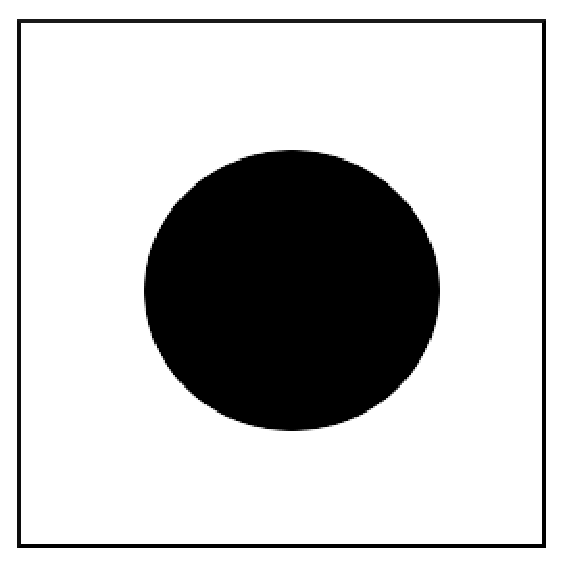
\includegraphics[scale=0.3]{images/circulo_250x250.eps}
\caption{Imagen artificial con bordes curvos entre clusters}
\label{fig:circulo}
\end{figure}

Las primeras pruebas para esta imagen consideran centroides iniciales aleatorios, y se trabajó nuevamente utilizando sólo las intensidades de gris primero y posteriormente incorporando las coordenadas de cada punto.

Los resultados obtenidos sin información espacial demuestran que el algoritmo es capaz de agrupar los puntos de manera correcta en zonas cerradas cuando existe un fuerte contraste de intensidades entre la zona interior y la exterior (figura \ref{fig:circulo_aleatorio} a y b). Al incluir las coordenadas espaciales los resultados obtenidos son diferentes. Si bien se logra diferenciar con claridad la zona central del fondo en la imagen original, se observa que las probabilidades de los puntos pertenecientes al cluster cerrado son afectadas por la distancia al centroide, que por lo que se puede observar, considerando que los puntos con valores de probabilidad más altos son los mas cercanos a éste, tiende a ubicarse en un punto tangente a la circunferencia (figura \ref{fig:circulo_aleatorio} c y d)

\begin{figure}[h]
\centering
\includegraphics[scale=0.08]{images/circulo-001.jpg}
\caption{Mapas de pertenencia con centroides iniciales aleatorios. (a - b)  sin información espacial (c - d) con información espacial.}
\label{fig:circulo_aleatorio}
\end{figure}

En la primera representación con información espacial (figura \ref{fig:circulo_aleatorio} - c) se puede ver que el rango de probabilidades para la zona circular varía desde $0,5$ tendiendo a $1$, pero sin lograr probabilidades altas, y en la segunda imagen (figura \ref{fig:circulo_aleatorio}-d) abarca probabilidades menores a $0.5$, pero no hay probabilidades nulas. A partir de la variación de colores que representan el mapa probabilístico, se observa claramente que hay incertidumbre para identificar los puntos pertenecientes a la región cerrada, y que esta incertidumbre aumenta en el resto de la imagen. Se puede apreciar además cómo las probabilidades en el fondo prácticamente recorren el rango completo, lo cual indica que la zona de fondo tampoco  es identificada con certeza como perteneciente a ningún cluster.

Luego se consideró la elección manual de los centroides iniciales: para uno de los clusters se ubicó en la zona central del círculo, mientras que para el otro fue seleccionado en el punto superior izquierdo de la imagen. No se evidencian diferencias en los resultados, y al igual que en el caso aleatorio, cuando se incluye información espacial los valores límites de probabilidades se desplazan hacia un punto tangente del objeto cerrado (figura \ref{fig:circulo_aleatorio_centr_manual}).

\begin{figure}[h]
\centering
\includegraphics[scale=0.08]{images/circulo-001.jpg}
\caption{Matriz de pertenencia, con centroide seleccionado manualmente. (a-b) sin información espacial. (c-d) con información espacial}
\label{fig:circulo_aleatorio_centr_manual}
\end{figure}

Al advertir que el resultado final era el mismo que con los centroides aleatorios,  se realizó el experimento de ejecutar el algoritmo con los centroides elegidos a mano pero con un límite de iteraciones acotado para observar cómo se desplazaban los mismos conforme las iteraciones avanzan. Como se aprecia en la figura \ref{fig:circulo_iteraciones}, inicialmente la circunferencia tiene valores cercanos a $0\%$ de pertenencia (figura \ref{fig:circulo_iteraciones}-a), pero los mismos aumentan a medida que se ejecutan más iteraciones, hasta llegar al resultado final (figura \ref{fig:circulo_iteraciones}-e), que coincide con el presentado en la figura \ref{fig:circulo_aleatorio_centr_manual}. A medida que el algoritmo progresa, el centroide se desplaza hacia un punto del borde de la circunferencia. También se puede ver que la región del fondo no logra ser identificada por el algoritmo, ya que las probabilidades abarcan el rango completo de 0 a 1. 

\begin{figure}[h]
\centering
\includegraphics[scale=0.08]{images/circulo_iteraciones_x1.jpg}
\caption{Matriz de pertenencia al primer cluster, con información espacial y selección manual de centroides iniciales. (a)Luego de 1 iteración, (b) luego de 10 iteraciones, ( c) luego de 25 iteraciones, (d) luego de 50 iteraciones, (e) luego de 100 iteraciones}
\label{fig:circulo_iteraciones}
\end{figure}

\subsection{Imágenes con ruido}
La siguiente serie de experimentos considera imágenes con ruido sal y pimienta. En la primera evaluación se utilizó una imagen con 1\% de ruido y luego se elevó al 30\% (figura \ref{fig:mitad_mitad_ruido_1p}).

\begin{figure}[H]
\centering
\includegraphics[scale=0.06]{images/original_mitad_con_ruido_1y30.jpg}
\caption{Ruido sal y pimienta 1\%}
\label{fig:mitad_mitad_ruido_1p}
\end{figure}

En caso de no incluir las coordenadas espaciales, los puntos de ruido son clasificados con una probabilidad baja de pertenencia a su clúster, debido a la diferencia de intensidad (figura \ref{fig:ruido_1y30}-a). El efecto se profundiza cuando analizamos una imagen con mayor presencia de ruido (figura \ref{fig:ruido_1y30}-b).


\begin{figure}[h]
\centering
\includegraphics[scale=0.055]{images/mitad_mitad__ruido_1y_30.jpg}
\caption{Matriz de pertenencias del cluster 1, sin información espacial. (a) con 1\% de ruido, (b) con 30\% de ruido
}
\label{fig:ruido_1y30}
\end{figure}

Contrariamente, cuando se añaden las coordenadas espaciales como otra característica al algoritmo, se obtiene una distribución general de probabilidades similar a la lograda para la imagen sin ruido (Figura \ref{fig:mitad_mitad_ruido_zoom} b-1), y al igual que en el experimento sin información espacial, los puntos con ruido son clasificados con menor probabilidad. 
En este caso, si comparamos en detalle las probabilidades obtenidas con y sin la información espacial, podemos observar que la probabilidad de pertenencia de los  puntos con ruido es más acertada cuando se utilizan las coordenadas del punto como característica adicional (Figuras \ref{fig:mitad_mitad_ruido_zoom} a-2 y b-2).


\begin{figure}[H]
\centering
\includegraphics[scale=0.05]{images/mitad_mitad_ruido_zoom-001.jpg}
\caption{Matriz de pertenencia al cluster 1, de la imagen con 1\% de ruido. 
(a-1) sin información espacial (a-2) acercamiento de región marcada en (a-1)
(b-1) con información espacial (b-2) acercamiento de región marcada en (b-1)}
\label{fig:mitad_mitad_ruido_zoom}
\end{figure}

\subsection{Imágenes con bias}
En las siguientes pruebas utilizamos una imagen con 3 regiones, correspondientes al fondo y a un objeto circular y un anillo alrededor del mismo que presentan bias (figura \ref{fig:circulo_bias}). El bias es una distorsión de la imagen causada por el instrumento de captura. Esta distorsión se presenta generalmente sobre los bordes de los objetos y causa cambios en la intensidad de los píxeles, de manera que el mismo tejido es representado por diferentes valores en la imagen \citep{juntu2005bias}.

\begin{figure}[H]
\centering
\includegraphics[scale=0.3]{images/biasing.png}
\caption{Imagen de bordes curvos con 3 clusters y bias}
\label{fig:circulo_bias}
\end{figure}

El comportamiento del algoritmo cuando no se utilizan coordenadas espaciales es similar al observado en las pruebas anteriores, las tres zonas fueron correctamente detectadas y se puede notar como el bias afecta las probabilidades de las zonas debido al cambio de intensidades  (figura \ref{fig:matriz_circulo_bias}).

\begin{figure}[H]
\centering
\includegraphics[scale=0.3]{images/bias_sin_coord.jpg}
\caption{Mapas de pertenencia sin información espacial (a) fondo (b) anillo ( c) centro}
\label{fig:matriz_circulo_bias}
\end{figure}

Cuando utilizamos coordenadas espaciales para la clasificación de esta imagen, podemos apreciar que, al igual que en los experimentos anteriores, el algoritmo no detecta correctamente la zona del fondo (figura \ref{fig:matriz_circulo_bias_espacial} a y b). En el caso particular de la imagen para el clúster del centro (figura \ref{fig:matriz_circulo_bias_espacial} - c), vemos concretamente la influencia de las coordenadas espaciales, ya que la zona central y el anillo que la rodea son reconocidos prácticamente como un solo grupo, pese a la diferencia de intensidades.

\begin{figure}[H]
\centering
\includegraphics[scale=0.3]{images/bias_con_coord.jpg}
\caption{Mapas de pertenencia con información espacial (a) cluster del fondo, zona izquierda (b) cluster del fondo, zona derecha  (c) centro}
\label{fig:matriz_circulo_bias_espacial}
\end{figure}

\subsection{Imágenes con bias y ruido}

En nuestra última prueba utilizamos una imagen con bias y ruido. En esta situación, la clusterización resultante es de menor calidad que en los experimentos anteriores debido a la presencia de una alto porcentaje de ruido así como un biasing pronunciado. 

\begin{figure}[H]
\centering
\includegraphics[scale=0.3]{images/biasing_con_ruido.png}
\caption{Imagen con bias y ruido}
\label{fig:circulo_bias_ruido}
\end{figure}

En los mapas de pertenencia de la figura \ref{fig:circulo_bias_ruido_cluster} se puede apreciar que, pese al ruido y al bias, el fondo de la imagen es correctamente clasificado (figura \ref{fig:circulo_bias_ruido_cluster}-a), pero en el segundo y tercer mapa el anillo y la parte central de la imagen original no son claramente distinguidos (figura \ref{fig:circulo_bias_ruido_cluster} b y c). Las pertenencia de la zona central y el anillo varían entre 0 y 1 y además se mezclan en determinadas zonas.

\begin{figure}[H]
\centering
\includegraphics[scale=0.3]{images/bias_sin_coord_con_ruido.jpg}
\caption{Mapa de pertenencia sin información espacial (a) cluster del  fondo (b) centro 1 (c) centro 2}
\label{fig:circulo_bias_ruido_cluster}
\end{figure}

\subsection{Análisis de costo y convergencia}
En todos los casos analizados, la curva de convergencia de la función costo tiene la forma mostrada en la Figura 17. Siempre hay un periodo inicial con un valor alto de la función costo y luego un punto de inflexión a partir del cual desciende abruptamente y los valores oscilan levemente hasta que el algoritmo se detiene, como se mencionó en la sección \ref{Introduccion}.

\begin{figure}[h]
\centering
\includegraphics[scale=0.3]{images/FALTA.png}
\caption{Curva de convergencia}
\label{fig:convergencia}
\end{figure}


\section{Extracción de mallas}
\section{Modelos deformables}
\subsection{Explicación de modelos deformables}
\subsection{Estudio de sensibilidad}
\chapter{Resultados}\label{chap:resultados}
En este capítulo se presentan los resultados obtenidos al evaluar el esquema de segmentación propuesto sobre imágenes de prueba. El mismo consiste en un subconjunto de MRI de cerebro extraídas de un \emph{datase}t ampliamente utilizado en el estado del arte, sobre las cuales se evaluó la capacidad del método de segmentación para detectar materia gris , materia blanca y líquido cefalorraquídeo. La evaluación de diversas características morfológicas de estos tejidos resulta de vital importancia en numerosas aplicaciones, incluyendo el diagnóstico de enfermedades cerebrales tales como el Alzheimer o la esclerosis múltiple \citep{kovacevic2002robust}.

El algoritmo fue evaluado tanto desde un punto de vista cuantitativo como cualitativo. Cuantitativamente, se estudió la capacidad del método para segmentar los tejidos anteriormente mencionados, comparando las mallas obtenidas con las segmentaciones de referencia disponibles en el \emph{dataset}, por medio de indicadores apropiados. Durante el estudio cualitativo, además, se contrastaron los datos numéricos con lo observado visualmente, y se analizaron cuestiones relativas a la calidad de las mallas resultantes, al aspecto visual de las mismas, y a diversas particularidades que se presentaron en algunos de los casos de estudio.

En la Sección \ref{section:datos_usados} se presentan los materiales a los cuales se les aplicó el esquema propuesto. En la Sección \ref{section:metricas_calidad} se introducen las métricas de evaluación utilizadas en el análisis cuantitativo. En la Sección \ref{section:evaluacion_cuantitativa} se exponen los resultados de la evaluación cuantitativa utilizando el indicador presentado en la Sección \ref{section:metricas_calidad} y finalmente en la Sección \ref{section:evaluacion_cualitativa} se muestra el análisis cualitativo.

\section{Materiales}\label{section:datos_usados}
Como se mencionó, se estudió la capacidad del algoritmo para la identificación y correcta segmentación de los tres principales tejidos cerebrales: materia blanca  (MB), materia gris (MG) y líquido cefalorraquídeo (LC).

Las imágenes utilizadas son un subconjunto de 9 resonancias magnéticas correspondientes al \emph{dataset Internet Brain Segmentation Repository} (IBSR), liberado por el Center for Morphometric Analysis del Massachusetts General Hospital con el objetivo de proveer un conjunto de datos estándar para la evaluación de algoritmos de segmentación de tejidos cerebrales \citep{rohlfing2012image, valverde2015comparison}. Tradicionalmente conocido en la literatura como IBSR18, el \emph{dataset} está compuesto por 18 MRIs modalidad T1-w de sujetos sin ninguna patología, con una distancia inter-slide de 1.5 mm y una resolución de 256 x 128 x 256 vóxeles, provistas en formato NIfTI-1. En la Figura \ref{fig:ISBR18} se presenta, a modo de ejemplo, un corte de cada uno de los 9 estudios seleccionados para la evaluación del algoritmo. Según puede observarse, el cráneo ha sido removido de las imágenes para evitar errores en la segmentación. Por otro lado, cabe destacar la variabilidad que existe entre las imágenes, en lo que respecta a artefactos, distribución de las intensidades, presencia y ausencia de bordes, ruido, etc. Esto permitió estudiar la capacidad del algoritmo para lidiar con la multiplicidad de casos que puedan llegar a presentarse en la práctica clínica.

\begin{figure}[H]
	\centering
	\includegraphics[scale=0.6]{images/IBSRsx9.jpg}
	\caption{Cortes de las MRI de IBSR18 utilizadas para la evaluación del método de segmentación propuesto.}
	\label{fig:ISBR18}
\end{figure}

El conjunto de datos provee también volúmenes de referencias, también denominados \emph{ground truths} (GT), como el que se observa en la Figura \ref{fig:GT}(b) para una de las imágenes, los cuales son utilizados en la comunidad científica para la evaluación de resultados. Cada imagen posee uno de estos volúmenes asociado, en donde la MB, la MG, el LC y el fondo se representan con intensidades bien diferenciadas. Así, resulta muy sencillo elaborar por umbralado las máscaras binarias correspondientes a cada tejido (Figura \ref{fig:GT}(b)). A partir de estas máscaras es que se extraen las mallas de superficie que luego son utilizadas para realizar la comparación con la segmentación obtenida utilizando el indicador presentado en la Sección \ref{section:metricas_calidad}.

\begin{figure}[H]
	\centering
	\includegraphics[scale=0.06]{images/IBSRvsGT.jpg}
	\caption{(a) corte axial de la imagen IBSR07 (b) Máscaras binarias correspondiente al GT asociado (en rojo la materia blanca, en verde el LC y en azul la MG)}
	\label{fig:GT}
\end{figure}

\section{Metricas de evaluación de calidad}\label{section:metricas_calidad}
Para evaluar cuantitativamente la calidad de las mallas obtenidas, se realizó una comparación entre la malla resultante del esquema propuesto y la malla generada a partir de la segmentación de referencia. La técnica utilizada para realizar el cálculo de la diferencia entre las superficies utiliza un método basado en una aproximación discreta del volumen encerrado entre las mallas \citep{d2008indicador}.

Entonces, para estudiar los resultados obtenidos por el algoritmo se consideró el indicador de calidad de la segmentación conocido como coeficiente Dice, dado por la ecuación:
%
\begin{equation}
Q = \dfrac{V_{R}\bigcup V_{S}}{V_{R}\bigcap V_{S}}
\end{equation}
%
donde $V_{S}$ es el volumen encerrado por la superficie segmentada $S$ y $V_{R}$ es el encerrado por la superficie de referencia $R$. Esta métrica alcanza el valor 1 cuando ambos volúmenes coinciden, y es cercana a 0 cuando los volúmenes son completamente difusos. El cálculo numérico de la unión y la intersección del volumen encerrado por las superficies se realizó utilizando una implementación propia de un método basado en la discretización del espacio y el uso del test del rayo \citep{foley1994introduction, d2008indicador}. La estrategia consiste en la discretización de dos de las tres dimensiones de la imagen, generando una matriz de $ N \times M $ celdas, desde las cuales se disparan rayos paralelos entre sí. Estos rayos intersectan o no las superficies, generando una serie de segmentos como se muestra en la Figura \ref{fig:discretizacionvolumen}.

\begin{figure}[H]
\centering
\includegraphics[scale=0.7]{images/calculo_indicador.png}
\caption{Segmentos que atraviesan las dos mallas}
\label{fig:discretizacionvolumen}
\end{figure}

Para cada rayo, se suman las longitudes de los segmentos que atraviesan las mallas correspondientes a $V_{R}$ y $V_{S}$, según corresponda. Luego, esta suma por el área de la celda es una aproximación del volumen encerrado entre las dos mallas. Cuanto más granular es la discretización (es decir, celdas más pequeñas) el error de aproximación será menor.

\section{Evaluación cuantitativa}\label{section:evaluacion_cuantitativa}
Inicialmente se obtuvieron los resultados aplicando de manera aislada la primera parte del esquema de segmentación propuesto, basada en el algoritmo de Fuzzy C-Means (FCM). En todos los casos el método se corrió un máximo de 50 iteraciones, siempre que no se haya alcanzado la convergencia previamente. El valor $\epsilon$ de convergencia empleado fue de $1x10^{-4}$. Tanto la cantidad máxima de iteraciones como $\epsilon$ fueron escogidos conforme el análisis de sensibilidad expuesto en la Sección \ref{section:segmentacion_fuzzy}. Debido a que, como se mencionó en el capítulo correspondiente, la salida del FCM consiste en una segmentación difusa de cada tejido, se aplicó  el método de umbralado descrito en la Sección \ref{section:umbralado} sobre los resultados obtenidos. Posteriormente se generaron mallas de superficie a partir de cada umbralado tal como se explicó en la Sección \ref{section:extraccion_de_mallas}. Los valores de calidad resultantes fueron obtenidos comparando la malla de cada tejido con la correspondiente malla extraída a partir del volumen de referencia provisto en el \emph{dataset}.

Posteriormente se calcularon los indicadores sobre el pipeline completo del método propuesto en este trabajo. Las mallas extraídas a partir del volumen obtenido por umbralado sobre la matriz de probabilidades fueron deformadas utilizando el método de Superficies Activas, considerando para su evolución los mapas probabilísticos correspondientes a cada tejido. Los parámetros del método fueron seleccionados en base a un análisis cualitativo de la malla resultante utilizando una determinada configuración sobre una única imagen, comparándola con la malla obtenida luego del FCM, y posteriormente se ajustaron intentando mejorar el indicador cuantitativo para esa misma imagen. La configuración final obtenida fue fijada posteriormente para el resto de las imágenes del conjunto. Los parámetros que dieron mejores indicadores para cada tejido se presentan en la Tabla \ref{table:parametros_snakes}.

\begin{table}[h]
	\centering
	\begin{tabular}{c|cccccc}
		\multicolumn{1}{l|}{} & A y B & C & K & D & It & $\epsilon$ \\ \hline
		MB & 0.01 & 0.001 & 2 & 1 & 50 & 0.001 \\
		MG & 0.08 & 0.08 & 6 & 1 & 50 & 0.001 \\
		LC & 0.05 & 0.08 & 2 & 1 & 50 & 0.001
	\end{tabular}
	\caption{Parámetros para la ejecución del Snakes}
	\label{table:parametros_snakes}
\end{table}

En la Tabla \ref{table:resultados_gris}, Tabla \ref{table:resultados_blanca}, y Tabla \ref{table:resultados_liquido} se presentan los valores de coeficiente Dice obtenidos para la segmentación de MG, MB y LC respectivamente. Se plantearon diferentes experimentos, utilizando como descriptores de la imagen por un lado sólo las intensidades (FCM I), por otro lado las intensidades y la imagen convolucionada con un filtro gaussiano con valor de $\sigma = 2$ (FCM I+G(2)), y por último, las intensidades y la imagen convolucionada con el mismo filtro con $\sigma = 0.5$ (FCM I+G(0.5)). Tomando como base las mallas resultantes, se ejecutó el método de Snakes utilizando la información de la matriz de probabilidad correspondiente al tejido evaluado (SNK I, SNKI+G(0.5), SNKI+G(2)). Adicionalmente se ejecutó el algoritmo de Snakes sobre la información proveniente de la imagen, en lugar de la matriz de probabilidades.

\begin{table}[h]
	\resizebox{\textwidth}{!}{%
		\begin{tabular}{r|ccc|cccc}
			& \cellcolor[HTML]{93D092}FCM I & \cellcolor[HTML]{93D092}\begin{tabular}[c]{@{}c@{}}FCM\\ I+G(2)\end{tabular} & \cellcolor[HTML]{93D092}\begin{tabular}[c]{@{}c@{}}FCM\\ I+G(0.5)\end{tabular} & \cellcolor[HTML]{CBCEFB}SNK I & \cellcolor[HTML]{CBCEFB}\begin{tabular}[c]{@{}c@{}}SNK\\ I+G(2)\end{tabular} & \cellcolor[HTML]{CBCEFB}\begin{tabular}[c]{@{}c@{}}SNK\\ I+G(0.5)\end{tabular} & \cellcolor[HTML]{CBCEFB}\begin{tabular}[c]{@{}c@{}}SNK \\ Imagen\end{tabular}\\ \hline
			ISBR1 & 0.6681 & 0.6426 & 0.6732 & 0.7325 & 0.7056 & \textbf{0.7329} & 0.5939 \\
			ISBR2 & 0.7330 & 0.7016 & 0.7281 & \textbf{0.7453} & 0.7219 & 0.7427 & 0.5955 \\
			ISBR3 & 0.6893 & 0.6792 & 0.6868 & 0.7370 & 0.7261 & \textbf{0.7374} & 0.6279 \\
			ISBR4 & 0.6422 & 0.6954 & 0.6203 & 0.7038 & \textbf{0.7394} & 0.6896 & 0.6283 \\
			ISBR5 & 0.7131 & 0.6838 & 0.7053 & \textbf{0.7376} & 0.7154 & 0.7344 & 0.5403 \\
			ISBR6 & 0.6967 & 0.6579 & 0.6679 & \textbf{0.7401} & 0.6991 & 0.7364 & 0.4588 \\
			ISBR7 & 0.5576 & 0.5590 & 0.5483 & \textbf{0.6471} & 0.6254 & 0.6394 & 0.4625 \\
			ISBR8 & 0.5926 & 0.5968 & 0.5867 & \textbf{0.6890} & 0.6585 & 0.6790 & 0.4310 \\
			ISBR9 & 0.5395 & 0.5462 & 0.5340 & \textbf{0.6390} & 0.6121 & 0.6317 & 0.4343 \\ \hline
			Media & 0.6480 & 0.6403 & 0.6390 & \textbf{0.7079} & 0.6893 & 0.7026 & 0.5303 \\ \hline
			Desvio Estandar & 0.0698 & 0.0590 & 0.0698 & \textbf{0.0412} & 0.0460 & 0.0442 & 0.0839 \\ \hline
		\end{tabular}
	}
	\caption{Coeficientes Dice obtenidos para cada imagen de prueba, media y desvío estándar para la segmentación de la MG}
	\label{table:resultados_gris}
\end{table}


Tras la ejecución del algoritmo de Snakes utilizando los resultados del FCM con intensidades y con el filtro gaussiano para la segmentación de MG se observa que, para todos los casos, el indicador de calidad mejora. Para las pruebas efectuadas sobre las 9 imágenes se obtuvo un incremento promedio de 6 puntos porcentuales en la métrica del Snakes sobre el FCM solo con intensidades, un incremento promedio de 4.9 puntos porcentuales para la ejecución de Snakes sobre las intensidades junto con el filtro gaussiano con $\sigma = 2$ y un aumento de 6.3 puntos porcentuales, en promedio, para el Snakes aplicado sobre los resultados del FCM con intensidades más el filtro gaussiano con $\sigma = 0.5$. Adicionalmente, los desvíos son menores en todos los casos para las ejecuciones de Snakes respecto a sus correspondientes corridas de FCM. Esto indica una menor variabilidad de los resultados, generando valores dentro de un rango acotado. Otro indicador positivo es el hecho de que, inclusive al utilizar los mismos parámetros para todas las imágenes, se observa una reducción del desvío, lo que indica que los resultados son estables sin necesidad de una adaptación de los parámetros a cada imagen en particular. 

También se puede apreciar que en los casos en los que el FCM dio indicadores bajos, como en las imágenes IBSR7, 8 y 9, la mejora obtenida con Snakes supera los 9 puntos. Esto señala una tendencia del modelo de Snakes a mejorar mallas de baja calidad, como las que en estos casos fueron generadas desde el FCM.

\begin{figure}[H]
	\centering
	\includegraphics[scale=0.5]{images/BoxPlotMG.png}
	\caption{Boxplot presentando la distribución estadística  de los indicadores calculados para la segmentación de la MG, para todas las configuraciones del método seleccionadas.
		}
	\label{fig:boxplotMG}
\end{figure}

En la Figura \ref{fig:boxplotMG} se presenta un análisis sencillo sobre el comportamiento de los indicadores de calidad para la segmentación de MG para cada método. El gráfico muestra que FCM tiene una varianza relativamente grande entre los distintos experimentos. Por el contrario, las tres primeras ejecuciones de Snakes, además de mejorar los indicadores en cada uno de los casos como se observó en la Tabla \ref{table:resultados_gris}, tienen una varianza más pequeña, logrando resultados más consistentes y dentro de un rango más acotado en relación a FCM.

\begin{table}[h]
	\resizebox{\textwidth}{!}{%
		\begin{tabular}{r|ccc|cccc}
			& \cellcolor[HTML]{93D092}FCM I & \cellcolor[HTML]{93D092}\begin{tabular}[c]{@{}c@{}}FCM\\ I+G(2)\end{tabular} & \cellcolor[HTML]{93D092}\begin{tabular}[c]{@{}c@{}}FCM\\ I+G(0.5)\end{tabular} & \cellcolor[HTML]{CBCEFB}SNK I & \cellcolor[HTML]{CBCEFB}\begin{tabular}[c]{@{}c@{}}SNK\\ I+G(2)\end{tabular} & \cellcolor[HTML]{CBCEFB}\begin{tabular}[c]{@{}c@{}}SNK\\ I+G(0.5)\end{tabular} & \cellcolor[HTML]{CBCEFB}\begin{tabular}[c]{@{}c@{}}SNK \\ Imagen\end{tabular} \\ \hline
			ISBR1 & \textbf{0.7542} & 0.7219 & 0.7527 & 0.7320 & 0.6957 & 0.7286 & 0.5617 \\
			ISBR2 & \textbf{0.8131} & 0.7875 & 0.8127 & 0.7880 & 0.7547 & 0.7858 & 0.6082 \\
			ISBR3 & \textbf{0.7729} & 0.7502 & 0.7689 & 0.7470 & 0.7158 & 0.7410 & 0.5684 \\
			ISBR4 & 0.7653 & 0.7680 & \textbf{0.7690} & 0.7463 & 0.7334 & 0.7453 & 0.6016 \\
			ISBR5 & \textbf{0.7673} & 0.7345 & 0.7646 & 0.7455 & 0.7110 & 0.7423 & 0.5596 \\
			ISBR6 & \textbf{0.7469} & 0.7022 & 0.7229 & 0.7302 & 0.6922 & 0.7146 & 0.5360 \\
			ISBR7 & \textbf{0.7964} & 0.7524 & 0.7871 & 0.7741 & 0.7190 & 0.7648 & 0.6324 \\
			ISBR8 & \textbf{0.8062} & 0.7737 & 0.8030 & 0.7827 & 0.7357 & 0.7772 & 0.5927 \\
			ISBR9 & \textbf{0.7784} & 0.7348 & 0.7708 & 0.7559 & 0.7011 & 0.7478 & 0.6050 \\ \hline
			Media & \textbf{0.7779} & 0.7472 & 0.7724 & 0.7557 & 0.7176 & 0.7497 & 0.5851 \\ \hline
			Desvio Estandar & 0.0229 & 0.0269 & 0.0267 & 0.0212 & \textbf{0.0206} & 0.0227 & 0.0304 \\ \hline
		\end{tabular}
	}
	\caption{Coeficientes Dice, media y desvío estándar para la segmentación de la materia blanca
		}
	\label{table:resultados_blanca}
\end{table}

En contraste con los resultados obtenidos para la MG, para la MB no se lograron mejoras respecto del resultado del FCM al ejecutar Snakes, como se puede observar en la Tabla \ref{table:resultados_blanca}. Además, para la ejecución basada únicamente en las intensidades se observa un decremento promedio de 2 puntos para el caso de las intensidades y un decremento de 3 puntos para los dos casos donde se utilizó el filtro gaussiano. Si se observa la Figura \ref{fig:boxplotMB}, se puede advertir en este caso una menor varianza de los indicadores para la ejecución de FCM para la segmentación de MB, comparada con la Figura \ref{fig:boxplotMG}. Una situación similar ocurre para las distintas opciones de ejecución del Snakes.

Analizando estos dos experimentos, los resultados parecieran indicar que Snakes tiene una mejor performance al trabajar sobre mallas de baja calidad (como en el caso de MG), y logra adaptarlas mejor utilizando el mapa probabilístico. Contrariamente, Snakes tiene dificultades para lograr mejoras sobre un malla que ya se puede considerar de buena calidad, como sucede en este experimento para MB.

\begin{figure}[H]
	\centering
	\includegraphics[scale=0.5]{images/BoxPlotMB.png}
	\caption{Boxplot presentando la distribución estadística de los indicadores calculados para la segmentación de la materia blanca, para todas las configuraciones del método seleccionadas.}
	\label{fig:boxplotMB}
\end{figure}


Como muestra la Tabla \ref{table:resultados_liquido}, tanto el FCM como el Snakes mostraron valores de calidad muy bajos para la segmentación del líquido cefalorraquídeo, lo que también puede apreciarse a partir de la Figura \ref{fig:boxplotLC}, en la cual se muestran además los valores altos de varianza  para las imágenes procesadas.  Estos resultados pueden ser causados por las diferencias de la clasificación del líquido cefalorraquideo sulcal (sCSF) en la segmentación de referencia. En general, los métodos tienden a clasificar los vóxeles de sCSF como líquido cefalorraquídeo. Sin embargo, los mismos están segmentados dentro del área gris en el \emph{ground truth} \citep{valverde2015comparison}. En este trabajo también  se obtienen resultados igualmente bajos para la segmentación del líquido cefalorraquideo utilizando diferentes algoritmos y proponen un pre procesamiento para quitar el sCSF y obtener mejores resultados al comparar con el volumen de referencia.

\begin{table}[h]
	\centering
	\resizebox{\textwidth}{!}{%
		\begin{tabular}{r|ccc|cccc}
			& \cellcolor[HTML]{93D092}FCM I & \cellcolor[HTML]{93D092}\begin{tabular}[c]{@{}c@{}}FCM\\ I+G(2)\end{tabular} & \cellcolor[HTML]{93D092}\begin{tabular}[c]{@{}c@{}}FCM\\ I+G(0.5)\end{tabular} & \cellcolor[HTML]{CBCEFB}SNK I & \cellcolor[HTML]{CBCEFB}\begin{tabular}[c]{@{}c@{}}SNK\\ I+G(2)\end{tabular} & \cellcolor[HTML]{CBCEFB}\begin{tabular}[c]{@{}c@{}}SNK\\ I+G(0.5)\end{tabular} & \cellcolor[HTML]{CBCEFB}\begin{tabular}[c]{@{}c@{}}SNK \\ Imagen\end{tabular} \\ \hline
			ISBR1 & 0.1914 & 0.1919 & \textbf{0.1957} & 0.1832 & 0.1755 & 0.1871 & 0.0981 \\
			ISBR2 & 0.3085 & \textbf{0.3107} & 0.3047 & 0.2805 & 0.2745 & 0.2784 & 0.1283 \\
			ISBR3 & 0.1332 & \textbf{0.1667} & 0.1401 & 0.1362 & 0.1564 & 0.1413 & 0.0297 \\
			ISBR4 & 0.0839 & \textbf{0.1285} & 0.0821 & 0.0809 & 0.1156 & 0.0798 & 0.0518 \\
			ISBR5 & 0.3825 & \textbf{0.3859} & 0.3754 & 0.3458 & 0.3291 & 0.3372 & 0.0286 \\
			ISBR6 & 0.4512 & \textbf{0.4689} & 0.4491 & 0.4022 & 0.3927 & 0.4014 & 0.1296 \\
			ISBR7 & 0.0898 & \textbf{0.1741} & 0.1006 & 0.0949 & 0.1702 & 0.1082 & 0.0551 \\
			ISBR8 & 0.1465 & \textbf{0.2728} & 0.1520 & 0.1455 & 0.2601 & 0.1523 & 0.0881 \\
			ISBR9 & 0.1101 & \textbf{0.1909} & 0.1190 & 0.1109 & 0.1781 & 0.1196 & 0.0510 \\ \hline
			Media & 0.2108 & \textbf{0.2545} & 0.2132 & 0.1978 & 0.2280 & 0.2006 & 0.0734 \\ \hline
			Desvío Estándar & 0.1361 & 0.1144 & 0.1316 & 0.1168 & 0.0914 & 0.1122 & \textbf{0.0391} \\ \hline
		\end{tabular}
	}
	\caption{Coeficientes Dice, media y desvío estándar para la segmentación del líquido cefalorraquídeo}
	\label{table:resultados_liquido}
\end{table}

\begin{figure}[H]
	\centering
	\includegraphics[scale=0.5]{images/BoxPlotLC.png}
	\caption{Boxplot presentando la distribución estadística de los indicadores calculados para la segmentación de la líquido cefalorraquídeo, para todas las configuraciones del método seleccionadas.}
	\label{fig:boxplotLC}
\end{figure}

Según puede observarse en los indicadores de los tejidos MB y MG, donde se pudieron alcanzar valores altos de calidad, excepto algunos casos aislados, en general utilizando únicamente intensidades, se pudieron obtener valores de calidad superiores a los obtenidos combinando las intensidades con la imagen convolucionada con un filtro gaussiano. Incluso en los casos en los que se obtuvieron mejoras, las mismas no resultan en extremo significativas. Esto se puede ver en los indicadores de FCM para MB y de SNK para MG.

\section{Evaluación cualitativa}\label{section:evaluacion_cualitativa}
Para realizar el análisis cualitativo de las mallas generadas, se utilizó como referencia la imagen original y la matriz de probabilidades obtenida por FCM, correspondiente al tejido evaluado y la variante de descriptores empleada para obtener los mapas probabilísticos utilizando FCM (sólo intensidades, o intensidades combinadas con un filtro Gaussiano con $\sigma = 0.5$ u otro con $\sigma = 2$).
A modo de referencia, en la Figura \ref{fig:cualitativa_matrices} se puede observar el mismo corte axial, del IBSR 8, y de las matrices correspondientes a la MB obtenida con las diferentes configuraciones de FCM.

\begin{figure}[H]
	\centering
	\includegraphics[scale=0.08]{images/IBSR_vs_probx3-001.jpg}
	\caption{Corte axial de IBSR8. (a) imagen original, (b) matriz FCM I, (c) matriz FCM I+G(0.5), (d) matriz FCM I+G(2).}
	\label{fig:cualitativa_matrices}
\end{figure}

Según puede observarse en la figura, el mapa probabilístico obtenido por FCM utilizando solamente las intensidades representa con bordes bien definidos a la región de interés (MB). A medida que se aumenta el sigma del filtro Gaussiano, por otro lado, es posible percibir que los bordes comienzan a difuminarse. En la Figura \ref{fig:cualitativa_acercamiento} se presenta un acercamiento de la matriz generada utilizando únicamente intensidades, y el mismo corte de la matriz utilizando intensidades combinadas con filtro Gaussiano con sigma 2. En la misma es posible observar que existen regiones en las que dejan de distinguirse algunas concavidades, y los bordes pierden definición. Esta particularidad es sin duda la que causa una disminución de la calidad de las mallas obtenidas por FCM con filtro Gaussiano y las generadas con Snakes utilizando estas matrices para guiar a las fuerzas externas, respecto a las obtenidas cuando se trabaja solo en base a las intensidades.

\begin{figure}[H]
	\centering
	\includegraphics[scale=0.08]{images/acercamiento_prob_NF_vs_prob_GA2.jpg}
	\caption{Acercamiento de la matriz de probabilidades de MB para el IBSR8. (a) FCM I, (b) FCM  I+G(2).}
	\label{fig:cualitativa_acercamiento}
\end{figure}

Para analizar el comportamiento de Snakes sobre estas diferencias en la matriz de probabilidades, en la Figura \ref{fig:cualitativa_mb} se presentan las mallas para MB correspondientes al GT (rojo), al resultado de aplicar FCM con intensidades (verde) y FCM con intensidades y filtro Gaussiano con $\sigma = 2$ (amarillo), sobre el mismo corte y acercamiento presentados en las Figuras \ref{fig:cualitativa_matrices} y \ref{fig:cualitativa_acercamiento}. Como se esperaba, en el acercamiento se puede observar que la malla generada por FCM I+G(2) pierde detalles sobre los bordes, alejándose de los mismos, respecto a la malla obtenida con FCM con intensidades, y en particular en el acercamiento se puede ver que la malla de FCM I+G(2) (amarilla) se separa en la sección central donde tanto la malla de GT (roja), como la de FCM I (verde), se mantienen unidas.

\begin{figure}[H]
	\centering
	\includegraphics[scale=0.08]{images/MB_1.jpg}
	\caption{Mallas para la MB del IBSR 8 sobre matriz de probabilidades de FCM con intensidades. Malla de GT(rojo)  y malla obtenidas con FCM I (verde) y con FCM  I+G(2) (amarilla).}
	\label{fig:cualitativa_mb}
\end{figure}

Con el objetivo de evaluar cualitativamente la calidad de las mallas obtenidas para los diferentes tejidos del cerebro, a continuación se muestran varios cortes para los experimentos con FCM y Modelos Deformables. Dado que los mejores resultados se alcanzan con las matrices de probabilidades generadas utilizando FCM con intensidades, el siguiente análisis se realizará únicamente sobre mallas obtenidas con FCM con intensidades y Snakes guiados por estas matrices.

\subsection{Materia Blanca}
En la figura \ref{fig:cualitativa_mb_2}, se puede observar un corte axial de las mallas correspondientes a la MB de la IBSR1, sobre la matriz de probabilidades (Figura \ref{fig:cualitativa_mb_2}(b)) y sobre la imagen original (Figura \ref{fig:cualitativa_mb_2}(c)). Como se puede observar, la malla generada por FCM (azul) se aproxima muy bien a la región de interés. Al definir los parámetros para el algoritmo de Snakes, se buscó propiciar cambios mínimos que permitan que la malla avance mejor sobre aquellos bordes que no se habían alcanzado. 


\begin{figure}[H]
	\centering
	\includegraphics[scale=0.08]{images/MB_2.jpg}
	\caption{Mallas de GT (rojo), obtenida por FCM (azul) y Snakes (verde) correspondientes a la MB para el IBSR1. (a) Acercamiento esquina superior izquierda del corte (b) Mallas sobre matriz de probabilidades obtenida por FCM I (c) Mallas sobre IBSR}
	\label{fig:cualitativa_mb_2}
\end{figure}

Por ejemplo, en el acercamiento (Figura \ref{fig:cualitativa_mb_2}(a)), se ve que la malla generada por Snakes (verde) se adapta mejor a la concavidad que se observa en la imagen. 
Si bien a simple vista la malla generada con Snakes pareciera mejorar con respecto a la obtenida con FCM, el indicador de calidad obtenido tiene un valor menor. Esto sucede porque, si comparamos con el GT (rojo), en muchos casos el resultado (verde) se aleja de dicha malla.

En la Figura \ref{fig:cualitativa_mb_3} se muestra un corte coronal para las mallas obtenidas, también para MB, para la imagen IBSR 6, en este caso se observa que en general, la malla obtenida mediante Modelos Deformables (verde) se acerca más hacia los bordes respecto a la obtenida por FCM (azul). Sin embargo, en muchos casos, también se aleja de lo definido en el GT (roja). En esta imagen también se aprecia que la malla asociada al GT (roja) tiene dos concavidades, indicadas con el recuadro amarillo, que no se pueden discriminar utilizando únicamente las intensidades de la imagen. Descriptores más complejos que puedan caracterizar ese sector mejorarían las matrices de probabilidad y, por consiguiente, permitirían obtener mejoras utilizando Snakes.

\begin{figure}[H]
	\centering
	\includegraphics[scale=0.4]{images/MB_3.jpg}
	\caption{Mallas de GT (rojo), obtenida por FCM (azul) y Snakes (verde) correspondientes a la MB para el IBSR6. (a) Sobre matriz de probabilidades obtenida por FCM I (b) Sobre IBSR}
	\label{fig:cualitativa_mb_3}
\end{figure}

\subsection{Materia Gris}
Sobre el corte sagital del IBSR9 (Figura \ref{fig:cualitativa_mg}), se puede ver que la malla de GT (roja) se encuentra considerablemente por fuera de lo que se clasifica como MG según la matriz de probabilidades obtenida por FCM (Figura \ref{fig:cualitativa_mg}(a)). Si bien la malla obtenida por FCM (azul) se encuentra bien ajustada al contorno de la región de interés, al observar que los indicadores de calidad no resultan altos, se decidió recalibrar los parámetros para mejorar con la etapa de Snakes. En este caso, incrementando la influencia de la fuerza de inflación y aumentando además el valor de K para permitir que la malla avance hacia valores más disímiles de probabilidad respecto a los de la región, los resultados obtenidos mejoran considerablemente. Este cambio se observa con claridad en la malla obtenida con Snakes (verde), que se aleja levemente del contorno de la matriz de probabilidades respecto de la posición inicial de la malla de FCM (azul), acercándose más a la malla de GT. 

\begin{figure}[H]
	\centering
	\includegraphics[scale=0.08]{images/MG_1.jpg}
	\caption{Mallas de GT (rojo), obtenida por FCM (azul) y Snakes (verde) correspondientes a la MG para el IBSR9. (a) Sobre matriz de probabilidades obtenida por FCM con intensidades (b) Sobre IBSR}
	\label{fig:cualitativa_mg}
\end{figure}

Algo interesante de analizar es que en todos los estudios considerados, en la segmentación de referencia se identifican como MG a regiones que ni con intensidades ni agregando el filtro gaussiano se pueden apreciar en las matrices de probabilidades obtenidas para dicho tejido (Figura \ref{fig:cualitativa_mg_2}, recuadros rojos). Sólo en ciertos casos, algunos puntos de esta región se identifican con una probabilidad relativamente alta. Por lo tanto, tampoco es posible mejorar la segmentación con Snakes para esta región, dado que se basa en la información de estas matrices para deformar la superficie activa.


\begin{figure}[H]
	\centering
	\includegraphics[scale=0.6]{images/MG_probVsGT.jpg}
	\caption{Corte Axial (A) y Coronal ( C) de las mallas GT para la MG (amarillo), sobre las matrices de probabilidades obtenidas con FCM para distintos IBSR.}
	\label{fig:cualitativa_mg_2}
\end{figure}

Dado que esto ocurre con todas las segmentaciones de referencia, es de suponer que se trataría de un tejido que es reconocido por el profesional médico utilizando conocimiento anatómico. La incorporación de otros indicadores más representativos, como se mencionó anteriormente, permitiría segmentar con más precisión la región correspondiente.

\subsection{Liquido Cefalorraquídeo}

En la Figura \ref{fig:cualitativa_lc}, se pueden ver las diferentes mallas para el LC en un corte axial de la IBSR5.  Para seleccionar los parámetros que mejoraran la calidad obtenida para las mallas de esta región, a diferencia de lo ocurrido con la MG, fue necesario disminuir la influencia de la fuerza de inflación y el valor de K, con el objetivo de impulsar a la malla a crecer únicamente en regiones con probabilidades muy similares a las de la región, y contraerse en caso contrario. Según puede observarse, la malla obtenida por Snakes (verde) se contrae levemente respecto de la obtenida por FCM (azul); sin embargo, en diversas regiones (recuadro naranja), la malla resultante sigue siendo considerablemente más grande que la malla de referencia (roja). Por otro lado, al disminuir la capacidad de inflarse de la malla ante probabilidades disímiles, en algunas regiones (recuadro amarillo) se dejan de detectar zonas que corresponden al tejido.

\begin{figure}[H]
	\centering
	\includegraphics[scale=0.5]{images/LC_1.jpg}
	\caption{Mallas de GT (rojo), obtenida por FCM (azul) y Snakes (verde) correspondientes al LC para el IBSR5. (a) Sobre matriz de probabilidades obtenida por FCM con intensidades (b) Sobre IBSR}
	\label{fig:cualitativa_lc}
\end{figure}

En la Figura \ref{fig:cualitativa_3dmagic} se presentan las reconstrucciones tridimensionales de las mallas obtenidas luego de aplicar FCM (azul) y el esquema completo (verde), superpuestas al GT de referencia.

\begin{figure}[H]
	\centering
	\includegraphics[scale=0.08]{images/mallas_3D.jpg}
	\caption{Mallas 3D de GT (rojo) superpuesta con FCM (azul) y GT con Snakes (verde), para la MB, MG y LC del IBSR2.
		}
	\label{fig:cualitativa_3dmagic}
\end{figure}

Para la MB se observa una superposición de las mallas con una predominancia superficial de la malla de FCM (azul) por sobre el GT (rojo). En la imagen correspondiente a Snakes (verde) se observa que la malla presenta una cantidad menor de falsos positivos que la obtenida por FCM.

De manera más acentuada, la misma observación se desprende de las mallas de la MG, donde vemos una predominancia superficial mucho mayor del GT al superponerlo con la malla obtenida con FCM, y no así en el caso de la resultante tras aplicar Snakes, donde se observa una segmentación más adaptada. También es posible notar como la tendencia inflacionaria del Snakes provoca menos falsos positivos, y, por lo tanto, una mejor adaptación a la malla del GT.  Nótese, además, que la aplicación de Snakes produce también un suavizado de la misma.

Para el LC observamos tanto para FCM como para Snakes una sobresegmentación superficial ya que las mallas verde y azul predominan sobre el rojo del GT.
\chapter{Conclusiones y trabajos futuros}
En el presente trabajo final de carrera se propuso un método para la segmentación de imágenes médicas tridimensionales basado en la integración de un algoritmo de clustering difuso (Fuzzy C-Means) con un esquema de Modelos Deformables. La combinación de ambas estrategias en un único pipeline de procesamiento permite principalmente la incorporación de información provista por múltiples descriptores al esquema de fuerzas de las Snakes. Para ello, se utiliza como entrada del modelo deformable el mapa de pertenencias correspondiente al tejido a segmentar, obtenido previamente haciendo uso del método de clustering. Esta integración permite incorporar multiplicidad de indicadores sin que sea necesario realizar mayores modificaciones al modelo original utilizado en la literatura. Por otro lado, esto permite hacer uso de una de las mayores ventajas del método de Snakes, que radica en la naturaleza conexa de la membrana deformable. Así, el método completo da lugar a una contribución al área de segmentación no supervisada que complementa ambas estrategias y realiza un aprovechamiento mayor de las características disponibles en la imagen.

Inicialmente se estudió el comportamiento del método de Fuzzy C-Means en diferentes condiciones de ruido y ante la presencia de artefactos característicos de las resonancias magnéticas tridimensionales. Durante estos estudios se demostró empíricamente que el método es capaz de diferenciar intensidades de manera correcta siempre y cuando las mismas no se vean afectadas de manera destacable por el ruido o presenten variabilidades tipo bias no muy pronunciadas. Se demostró, además, que la incorporación de las coordenadas de la imagen como descriptores, lejos de permitir mejorar estas dificultades, empeora notoriamente los resultados, concluyendo así que sería necesario realizar una modificación del modelo completo si se desea tener en cuenta esta información en esta etapa.

Posteriormente se propuso una estrategia de umbralado a partir de los mapas probabilísticos resultantes del algoritmo de Fuzzy C-Means, robusta a la presencia de ruido y que permite obtener mallas sin orificios. La misma consiste en asignarle a cada cluster la etiqueta correspondiente a aquel mapa en donde la probabilidad de pertenencia es mayor, y en un postprocesamiento adicional del volumen binario resultante para remover huecos.

En una tercera etapa, se desarrolló un algoritmo basado en Snakes que permite la deformación de las mallas obtenidas por Fuzzy C-Means, pero utilizando el mapa probabilístico correspondiente a la región de interés en lugar de las intensidades de la imagen. Se incorporó, además, un estudio de sensibilidad de los parámetros del modelo, con el objeto de analizar cómo la variación de cada uno de ellos afecta a los resultados finales.

El esquema completo de segmentación fue evaluado para la segmentación de materia blanca, materia gris y líquido cerebroespinal o cefalorraquideo a partir de un conjunto de imágenes MRI T1-w de cerebros sanos ampliamente utilizada en la literatura. Los valores de coeficiente Dice obtenidos fueron, en promedio, de 0.22 para el líquido cefalorraquideo, 0.70 para la materia gris y 0.75 para la materia blanca. 

Según pudo concluirse a partir del análisis cualitativo y cuantitativo de los resultados, el método es capaz de obtener resultados más que satisfactorios para la materia gris y la materia blanca, aunque los valores de calidad para el líquido cefalorraquídeo requieren ser todavía mejorados. Una posible causa de esta dificultad puede radicar en los propios datos utilizados para la evaluación, que, según se ha indicado en literatura reciente \citep{valverde2015comparison}, presenta algunos errores en el etiquetado. 

El método fue evaluado utilizando las intensidades de la imagen como descriptores de los píxeles, y las intensidades combinadas con los valores de gris obtenidos tras la convolución de la imagen con filtros gaussianos con diferente valor de sigma. Según pudo observarse, la incorporación de este indicador no mejora los resultados obtenidos respecto a la versión basada exclusivamente en intensidades. No es posible, sin embargo, concluir que esto sucede para todo tipo de indicadores, debido sobre todo a que los resultados combinando intensidades y gaussiano mejoran paulatinamente conforme se reduce el valor de sigma, algo que puede estar vinculado a la naturaleza difusa que presentan los bordes luego de aplicado el filtro. En un futuro se prevé la evaluación del pipeline completo pero haciendo uso de descriptores más robustos, tales como información de atlas, descriptores de textura, filtros de realce o indicadores creados ad-hoc para la exclusiva segmentación de tejidos cerebrales.

En general, se demostró también que el método de Snakes permite mejorar ampliamente los resultados obtenidos utilizando solamente Fuzzy C-Means para la segmentación de materia gris. En el caso de la materia blanca se observó una pequeña disminución, que se intuye está relacionada también con la poca capacidad para discriminar algunas regiones del cerebro utilizando únicamente intensidades. La integración de información relativa a la morfología de los tejidos permitiría, en un futuro, mejorar esta performance notoriamente.

Entre los trabajos futuros que pueden desprenderse de esta tesis de grado, uno de los más inmediatos debería basarse en la utilización de un algoritmo inicial más robusto que Fuzzy C-Means. En particular, la incorporación de los scores obtenidos mediante el uso de un clasificador supervisado (por ejemplo, Support Vector Machines) en reemplazo de los mapas probabilísticos permitiría mejorar los resultados en situaciones en las que los descriptores no llegan a ser tan certeros como es de esperar. Por otro lado, un análisis general y cualitativo del costo computacional del prototipo Matlab desarrollado para este trabajo sugiere el desarrollo futuro de mejoras basadas en cálculo paralelo, ya sea mediante el uso de múltiples threads a correr en los diferentes núcleos de la CPU, o bien la migración y paralelización de la implementación en GPUs.

Con posterioridad a la presentación de este trabajo se prevé, además, la puesta a disponibilidad del código fuente de este prototipo, a los efectos de contribuir con la comunidad de desarrolladores Matlab a través del sitio File Exchange de Mathworks.


%% Use letters for the chapter numbers of the appendices.
\appendix

\listoffigures
\listoftables
%% \input{appendix-a}

\bibliography{Bibliografia}

\end{document}
